Esamineremo ora alcuni modelli che sono stati costruiti per finalizzare la descrizione del nucleo.

Una classificazione di alcuni modelli nucleari in base al tipo di interazione tra nucleoni è la seguente:
\begin{multicols}{2}
	\begin{center}
		Models with strong interaction between nucleons:
	\end{center}
	\begin{itemize}
		\item \textbf{Liquid drop model} (Modello a goccia);
		\item \textbf{Shell model} (Modello a shell);
		\item $ \alpha-$particle model.
	\end{itemize}
   \begin{center}
	   Nucleons interact with the nearest neighbors and practically don‘t move: mean free path \[ \lambda \ll R\]
   \end{center}
	\columnbreak

	\begin{center}
		Models of non-interacting nucleons :
	\end{center}
	\begin{itemize}
		\item \textbf{Fermi gas model} (Modello a gas di fermioni);
		\item Optical model (Modello ottico).
	\end{itemize}
	\begin{center}
		Nucleons move freely inside the nucleus: mean free path \[ \lambda \sim R\]
	\end{center}
\end{multicols}
\begin{center}
($ R$ being the nuclear radius)
\end{center}
\section{Il modello nucleare a goccia}\label{sec:il-modello-nucleare-a-goccia}
Il grafico (Fig.~\ref{fig:en-legame-graph}) della energia di legame media per nucleone commentato in precedenza
contiene un certo numero di importanti indicazioni
sulle proprietà della forza nucleare che sono alla base di un primo
modello del nucleo - suggerito da Bohr nel 1935 - fondato essenzialmente
sul \textbf{raggio finito} della interazione nucleare.
Similmente alle forze intramolecolari a corto raggio nei liquidi,
tale fatto determina una certa analogia tra il comportamento dei nucleoni
nel nucleo e le diverse porzioni di un fluido meccanico incomprimibile, ragione che
giustifica il nome spesso usato di \textbf{modello a goccia}.
\begin{figure}
	\centering
	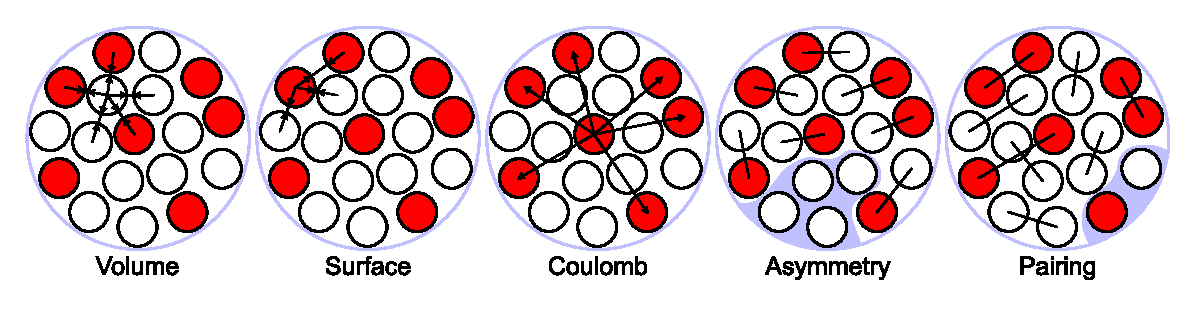
\includegraphics{figs/liquid-drop-model}
	\caption{Rappresentazione grafica del significato fisico dei termini presenti nel nuclear liquid drop model.}
	\label{fig:liquid-drop-model}
\end{figure}

Il suddetto modello ha base \textbf{fenomenologica}; la sola ipotesi
dell'andamento a corto raggio della forza non è sufficiente a
giustificare l'andamento reale

Come accennato, l'energia di legame tende ad assumere rapidamente il
valore medio di circa \(8MeV\) per nucleone (saturazione) il che indica
una energia di legame del nucleo proporzionale al numero di nucleoni
\begin{equation}
	\frac{B}{A} \simeq 8 MeV \qquad B \simeq 8 MeV \times A
    \label{eq:saturation-binding-energy-per-nucleon}
\end{equation}
Ora, se la forza nucleare si comportasse come una forza a lungo
raggio (come le forze gravitazionali o elettromagnetiche) ogni nucleone
interagirebbe con tutti i rimanenti altri per cui dovremmo attenderci
una energia di legame del nucleo tendenzialmente \emph{proporzionale al numero
di coppie} di nucleoni e dunque quadratica in A
\[
	B \propto \frac{A(A-1)}{2} \propto A^{2} \qquad
\]
Poiché i dati sulla energia di legame escludono questo tipo di
comportamento, dobbiamo concludere che ogni nucleone del nucleo
interagisce solo con un numero di fisso di nucleoni vicini per cui
concludiamo che \textbf{l'interazione forte ha un raggio d'azione finito}
dell'ordine di grandezza delle dimensioni del nucleone stesso.

Tale conclusione è in perfetto accordo con i dati sulla sezione d'urto
di neutroni su nuclei analizzati in precedenza che indicavano un \textbf{volume
nucleare proporzionale al numero di nucleoni}, ovvero una densità
volumetrica di nucleoni uniforme sul volume nucleare, fatto spiegabile
solo postulando la esistenza di una forza d'interazione tra nucleoni a
corto raggio.

Il primo tentativo di superare questo limite consiste nell'introdurre un
termine, sulla base della (\ref{eq:saturation-binding-energy-per-nucleon})
\begin{equation}
	B = a_{v} A
   \label{eq:volume-term-drop-model}
\end{equation}
dove la costante \(a_{v}\) viene detta \textbf{termine di volume}.
\begin{marginfigure}
	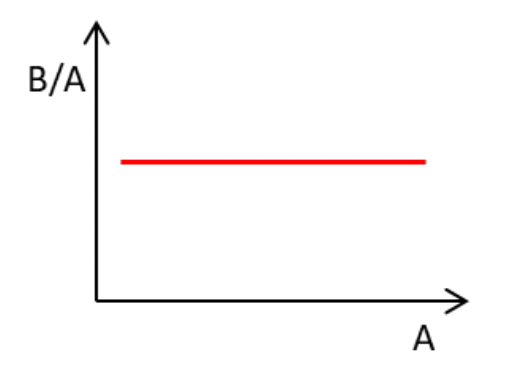
\includegraphics{figs/goccia1}
	%    \caption{This is a margin figure.}
	\label{fig:goccia1}
\end{marginfigure}
Con un tale andamento \(B / A\) , però, si finisce per ottenere una sovrastima
del volume.
La deviazione più rilevante si manifesta per valori piccoli di A dove
l'energia media di legame è molto inferiore a quanto previsto dalla
formula.
\bigskip

Si può allora osservare che, assumendo la forza nucleare a
corto raggio, si deve tenere conto che un nucleone prossimo alla
superficie del nucleo interagirà con un numero di nucleoni inferiore a
quello con cui interagirebbe qualora si trovasse all'interno del nucleo
stesso.
Ciò comporta che i nucleoni superficiali contribuiranno in
misura minore alla energia di legame nucleare di quelli interni al
volume.
Assumendo il nucleo di \textbf{forma sferica}, il numero di
nucleoni prossimi alla superficie sarà proporzionale a \(R^{2}\).
Dalla trattazione precedente (\ref{eq:nuclear-radius-skin}) sappiamo che (omettendo il termine di `skin'
nucleare) \begin{gather*}
	R_{\text{nuc}} = r_{0}A^{1/3}\\
	4 \pi R^{2} = 4 \pi (r_{0}A^{1/3})^2 \implies R_{\text{nuc}} \propto A^{2/3}
\end{gather*} per cui vi deve essere un termine che deve provocare un difetto di
energia di legame proporzionale ad \(A^{2/3}\): \[
	B = a_{v}A - a_{s}A^{2/3}
\] dove la costante \(a_{s}\) viene detta \textbf{termine di
	superficie}.
L'andamento di \(B / A\) con questa ulteriore correzione
può apprezzarsi a lato.
\begin{marginfigure}
	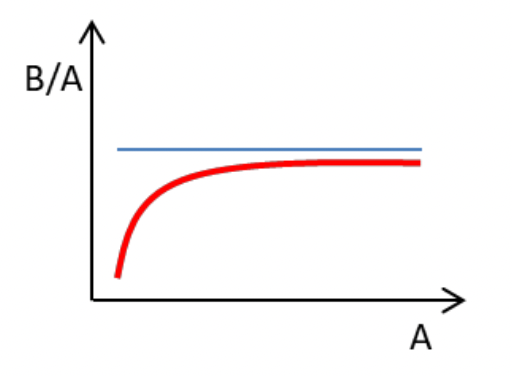
\includegraphics{figs/goccia2}
	%    \caption{This is a margin figure.}
	\label{fig:goccia2}
\end{marginfigure}
\bigskip

Un ulteriore miglioramento può essere ottenuto tenendo presente che i
protoni del nucleo si \emph{respingono elettrostaticamente} diminuendo
quindi il lavoro necessario per separarli dal nucleo stesso.
In effetti
se, per assurdo, si avesse un nucleo composto solo di protoni(senza
neutroni) il lavoro da spendere per mantenerne la configurazione sarebbe
sicuramente maggiore.

Ipotizzando una \emph{distribuzione di protoni uniforme} nel volume
nucleare (ricordiamo essere sferico dall'ipotesi precedente), otteniamo
la seguente espressione del lavoro fatto dalle forze coulombiane
repulsive per separare la carica nucleare
\begin{gather*}
	\delta L = \int _{R}^{\infty} \left( \frac{q \delta q}{4 \pi \epsilon_{0}r^{2}}  \hat{\bm{r}} \right)(dr \hat{\bm{r}})=
	- \frac{q \delta q}{4 \pi \epsilon_{0}r} \bigg |_{R}^{\infty} =
	- \frac{q \delta q}{4 \pi \epsilon_{0}R}\\
	q = \rho \frac{ 4}{3} \pi R^{3} \qquad \delta q = \rho 4 \pi R^{2} dR\\
	\delta L = \frac{1}{4 \pi \epsilon_{0}R}\left( \rho \frac{ 4}{3}\pi R^{3} \right)(\rho 4 \pi R^{2} dR) = \frac{4 \pi \rho^{2}}{3 \epsilon_{0}}R^{4}dR\\
	L = \int \delta l = \frac{4 \pi \rho^{2}}{15 \epsilon_{0}}R_{0}^{5} \qquad Q = \rho \frac{ 4}{3} \pi R_{0}^{3} = Ze\\
	L = \frac{3}{20 \pi \epsilon_{0}} \frac{Q^{2}}{R_{0}} = \frac{3e^{2}}{20 \pi \epsilon_{0}r_{0}} \frac{Z^{2}}{A^{1/3}}
	\implies L \propto \frac{ Z^{2}}{A^{1/3}}
\end{gather*} Ne consegue che la energia di legame nucleare dovrà essere corretta
sottraendo un termine proporzionale a \(Z^{2} / A^{1/3}\) per cui
l'espressione dell'energia di legame acquisirà la forma seguente
\begin{equation}
	B = a_{v}A - a_{s}A^{2/3} - a_{c} \frac{Z^{2}}{A^{1/3}}
	\label{eq:coulomb-term-drop-model}
\end{equation}
 dove la nuova costante \(a_{c}\) viene detta \textbf{termine
	coulombiano}.
Il termine coulombiano deve chiaramente annullarsi per
\(A=1\)(non c'e interazione elettrostatica) per cui l'unica forma
possibile è
\begin{equation}
	L \propto \frac{Z(Z-1)}{A^{1/3}} \quad
   \label{eq:work-to-seperate-uniformly-distributed-protons}
\end{equation}
\begin{marginfigure}
	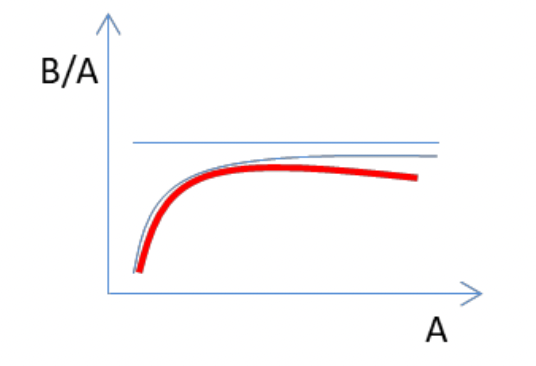
\includegraphics{figs/goccia3}
	%    \caption{This is a margin figure.}
	\label{fig:goccia3}
\end{marginfigure}

L'andamento $B / A$ risulta ulteriormente migliorato (si tenga presente
che nei nuclei stabili si ha approssimativamente \(Z=A/2\) per cui il
termine coulombiano sottrae un contributo crescente con \(A^{5/3}\)).

Se il modellino fenomenologico costruito finora fosse completo dovremmo
concludere che i nuclei più stabili(\(B= B_{max}\)) sono quelli con
\(Z=0\) ovvero i nuclei di soli neutroni.
Tale fatto è palesemente
contraddetto dai dati sperimentali i quali mostrano che i nuclei stabili
hanno un numero di protoni di poco inferiore a quello dei neutroni (la
differenza tra neutroni e protoni tende a crescere con il numero
atomico).
Il nostro modello -- basato sulla natura a corto raggio della
interazione nucleare -- non offre alcun appiglio per dare un fondamento
fisico a questo stato di cose che potrà essere spiegato solo nel
contesto della meccanica quantistica attraverso il \emph{principio di
	esclusione di Pauli}.
In questa situazione l'unica possibilità è quella
di introdurre un termine `ad hoc' capace di descrivere i dati
sperimentali.

Bisogna quindi fare in modo che il modello ci dica che i nuclei piu
stabili sono quelli con lo stesso numero di protoni e neutroni.
Raggiungiamo l'obiettivo introducendo un nuovo termine del tipo:
\[
	Z \simeq \frac{A}{2} \quad A - 2Z \simeq 0
\]
Ricordando però che con il crescere di \(A, Z\) tende ad essere via
via più piccolo di \(A/2\) (il quoziente protoni/neutroni diminuisce con
\(A\)), tale termine correttivo dovrà seguire una legge inversa ad A
modulata da un qualche esponente.
I dati indicano che la prima potenza è
sufficiente per cui abbiamo la seguente espressione della energia di
legame nucleare
\[
	B = a_{v}A - a_{s}A^{2/3} - a_{c} \frac{Z(Z-1)}{A^{1/3}} - \frac{a_{a}(A-2Z)^{2}}{A}
\]
dove la nuova costante \(a_{a}\) viene detta \textbf{termine di asimmetria}.
Notiamo che la presenza di \(A\) a denominatore è
giustificata osservando l'andamento dei dati sperimentali nel grafico
visto in precedenza:tanto piu \(A\) è grande tanto piu \(B / A\) devia
dalla tangente alla curva (quindi verso il basso).

Per completare il modello è necessario tenere conto di un ulteriore
proprietà dei nuclei.
I dati sperimentali mostrano che tra i 254 nuclei
stabili noti ben 148 sono del tipo \textbf{pari-pari} (un numero pari
sia di protoni che di neutroni), 101 sono del tipo \textbf{pari-dispari}
(un numero pari di protoni ma dispari di neutroni o viceversa) e solo 5
sono del tipo dispari-dispari (riportati in tabella \ref{tab:odd-odd-stable-nuclei}).
\begin{table}
	\centering
	\begin{tabular}{|c|}
		\hline
		$\isotope[2][1]{\mathlarger{H}}$ \\ \hline
		$\isotope[6][3]{\mathlarger{Li}}$ \\ \hline
		$\isotope[10][5]{\mathlarger{B}}$ \\ \hline
		$\isotope[14][7]{\mathlarger{N}}$ \\ \hline
		$\isotope[180m][73]{\mathlarger{Ta}}$ \\ \hline
	\end{tabular}
	\caption{Tabella dei nuclei stabili con both $ A,Z$ dispari. L'$m$ ad apice indica la metastabilità del nuclide. \\
	Si veda \url{https://en.wikipedia.org/wiki/Metastability#Nuclear_physics} a tale proposito.}
	\label{tab:odd-odd-stable-nuclei}
\end{table}

Similmente, tra i 35 nuclei a lunga vita media si hanno 22 pari-pari, 9 pari-dispari e 4
dispari-dispari.

Tali dati sembrano suggerire che per qualche motivo la forza forte tra
nucleoni da luogo a nuclei di maggiore stabilità quando vengono legati
\textbf{numeri pari} di neutroni e protoni, un fatto che trova una sua
diretta evidenza nell'andamento della energia di legame per nucleone
della serie isotopica dello xenon in Figura~\ref{fig:binding-energy-xenon}.
Tali dati sembrano suggerire che per qualche motivo la forza forte tra nucleoni da luogo a nuclei di maggiore stabilità
quando vengono legati \textbf{numeri pari} di neutroni e protoni, un fatto che trova una sua diretta evidenza nell’andamento della energia di legame per nucleone della serie isotopica dello xenon.
\begin{marginfigure}
	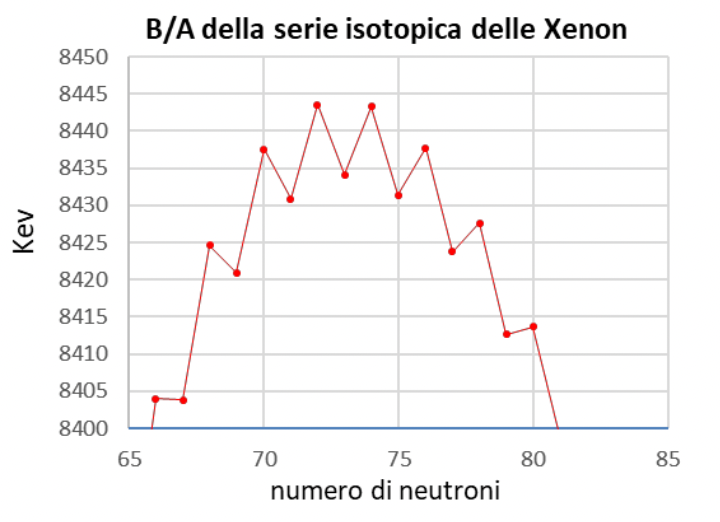
\includegraphics[scale = 1.5]{figs/goccia5}
	\caption{Andamento dell'energia di legame per la serie isotopica dello Xenon.}
	\label{fig:binding-energy-xenon}
\end{marginfigure}
Tenendo presente che il nucleo di Xenon ha \(Z=54\) protoni, si può
infatti constatare che gli isotopi con un numero pari di neutroni hanno
una maggiore energia di legame per nucleone.
Per rendere conto di questo
fatto si introduce un nuovo coefficiente detto di \textbf{pairing} \[
	a_{p} \frac{\delta}{A^{3/4}}
\] con \[
	\delta =
	\begin{cases}
		+1    \qquad  \text{pari-pari}       \\
		\ 0  \qquad  \ \ \text{pari-dispari} \\
		-1  \qquad  \text{dispari-dispari}
	\end{cases}
\] Giungiamo così alla seguente espressione complessiva della energia di
legame nucleare detta anche \textbf{formula semiempirica della energia
	di legame nucleare} o \textbf{formula di Weizsacker} della energia di
legame nucleare
\begin{equation}
	\boxed{    B = a_{v}A - a_{s}A^{2/3} - a_{c} \frac{Z(Z-1)}{A^{1/3}} - a_{a}\frac{(A-2Z)^{2}}{A} +     a_{p} \frac{\delta}{A^{3/4}}}
	\label{eq:weizsacker-formula}
\end{equation} Essa dipende da 5 parametri(vedi Fig.~\ref{fig:liquid-drop-model}) il cui valore numerico
viene determinato adattando la formula ai dati sperimentali di \(B/A\).

A titolo di esempio, una possibile combinazione di valori è la seguente (i
valori sono in \(MeV\)):
\begin{equation}
	a_{v} = 15.5 \quad a_{s} = 16.8 \quad a_{c} = 0.72 \quad a_{a} = 23.0 \quad a_{p} = 34.0
	\label{eq:typical-values-drop-model}
\end{equation}
La formula della energia di legame nucleare è utile - come strumento di
calcolo - perchè suggerisce una prima interpretazione del nucleo e delle
forze che lo tengono insieme.

Da essa deduciamo che le forze tra nucleoni devono essere \textbf{molto
	intense} ma a \textbf{short range} (proprietà di saturazione), producono
una distribuzione spaziale tendenzialmente uniforme di nucleoni e
conducono ad una espressione della energia di legame con termini di
volume e superficie in analogia con quanto accade per i liquidi, ragione
che giustifica il nome spesso usato di \textbf{modello nucleare a
	goccia}.

Il \emph{modello a gas di fermioni} (giustificabile con considerazioni
quantomeccaniche) riesce a rendere conto del termine \(a_{a}\) mentre
fallisce per quello di pairing.
Vedremo, infine, che il \emph{modello a shell} sarà quello piu preciso.

%%%%%%%%%%%%%%%%%%%%%%%%%%%%%%%%%%%%%%%%%%%%%%%%%%%%%%%%%%%%%%%%%%%%%%%%%%%%%%%%%%%%%%%%%%%%%%%%%%%%%%%%%%%%%%%%%%%%%%%%
%%%%%%%%%%%%%%%%%%%%%%%%%%%%%%%%%%%%%%%%%%%%%%%%%%%%%%%%%%%%%%%%%%%%%%%%%%%%%%%%%%%%%%%%%%%%%%%%%%%%%%%%%%%%%%%%%%%%%%%%
%%%%%%%%%%%%%%%%%%%%%%%%%%%%%%%%%%%%%%%%%%%%%%%%%%%%%%%%%%%%%%%%%%%%%%%%%%%%%%%%%%%%%%%%%%%%%%%%%%%%%%%%%%%%%%%%%%%%%%%%
\section{Il nucleo come gas di fermioni}\label{sec:il-nucleo-come-gas-di-fermioni}



Il modello a goccia del nucleo - essenzialmente fondato sulla natura a corto raggio delle interazioni forti - riesce a descrivere alcune proprietà del nucleo tra le quali l’esistenza di una energia di legame con termini di volume, superficie e coulombiano.
Non riesce invece a rendere conto in nessun modo dei termini di asimmetria e accoppiamento, chiaramente richiesti dai dati sperimentali, ma che devono essere introdotti ‘a mano’ nella formula di Weizsacker.
Tale fatto dimostra che oltre alla natura a corto raggio delle interazioni forti, nel nucleo giocano un ruolo di rilievo altre proprietà trascurate dal modello a goccia, presumibilmente legate alla natura quantomeccanica dei suoi costituenti.
Il modello nucleare a gas di fermioni introduce nel gioco alcuni essenziali proprietà quantomeccaniche in una forma il più possibile semplificata.

\subsection{Aspetti generali}\label{sec:aspetti-generali}

Le considerazioni fisiche che conducono alla formulazione del modello a gas di fermioni possono essere riassunte nei seguenti punti:
\begin{itemize}
	\item l’interazione forte che lega protoni e neutroni nel nucleo è a corto raggio
	e dell’ordine del raggio dei nucleoni stessi;
	\item ogni nucleone sarà quindi soggetto alla forza forte dei nucleoni
	immediatamente a contatto che tenderanno così a disporsi con densità
	volumetrica approssimativamente costante;
	\item ciò comporta che la risultante delle forze agenti sul singolo nucleone sia
	mediamente nulla quando questo si trova all’interno al nucleo e mediamente non nulla e diretta verso il centro quando questo si trova sulla superficie del nucleo;
	\item riassumersi in una forza dipendente dalla posizione, nulla all’interno di un volume sferico di raggio $R$ (raggio nucleare) e non nulla e centrale sulla sua superficie;
	\item essendo $ \bm{F} = - grad \, U$, tale forza può essere descritta da un potenziale
	nullo all’interno del volume sferico di raggio R, che sale con una certa ripidità in corrispondenza della superficie sferica,
	fino a raggiungere un valore costante al di fuori di essa. \\
	In sintesi, una \textbf{buca sferica di potenziale di raggio R} all’interno della quale vanno a collocarsi sia i neutroni che i protoni.
\end{itemize}
\bisgkip

Dato questo assetto delle forze, la meccanica quantistica fa il resto.
Infatti sappiamo che
\begin{itemize}
	\item una particella microscopica vincolata a rimanere in una regione di spazio
	limitata (nel nostro caso all’interno della buca di potenziale) deve annullare la propria funzione d’onda più o meno sulla superficie di tale regione ed all’esterno di essa;
	\item ciò comporta la quantizzazione delle lunghezze d’onda di De Broglie dei neutroni e dei protoni e, con esse, della loro energia (fenomeno analogo alla quantizzazione delle lunghezze d’onda in una corda vibrante) cosicchè gli stati quantomeccanici vanno a costituire una serie discreta e numerabile;
	\item dato che protoni e neutroni hanno spin $s=\frac{1}{2}$, essi vanno a costituire due insiemi di fermioni identici soggetti alle restrizioni del principio di esclusione;
	\item organizzando la serie discreta degli stati quantomeccanici possibili secondo i valori crescenti delle loro energie, il principio di esclusione permette di collocare in ciascuno di essi un solo protone ed un solo neutrone;
	\item nello stato fondamentale di minima energia del nucleo, neutroni e protoni nucleari riempiranno allora dal basso tutti gli stati quantomeccanici fino ad un livello energetico massimo detto \textbf{livello di Fermi} (nello stato fondamentale di minima energia dunque, i neutroni ed i protoni non sono immobili ma possiedono una certa energia cinetica crescente).
\end{itemize}

Le precedenti considerazioni ci conducono a concludere che la \emph{natura della forza media nucleare}, combinata con la
\emph{natura quantomeccanica dei suoi costituenti}, \textbf{assimila il nucleo nel suo stato fondamentale ad un doppio
gas di neutroni e protoni in condizioni di massima degenerazione}.
Parliamo di `gas’ poiché neutroni e protoni – come si è detto – si muovono essenzialmente liberi all’interno del volume nucleare subendo le sole forze di contenimento delle pareti nucleari.
Il termine ‘doppio’ ricorda che le restrizioni del principio di esclusione si applicano separatamente ai protoni ed ai neutroni.
Infine, il termine ‘degenerazione’ si riferisce al fatto che gli stati quantomeccanici quantizzati si riempiono tutti a partire da quelli meno energetici fino al livello di Fermi.
Come noto, tale condizione si realizza nei \textbf{gas di fermioni identici alle bassissime temperature che trovano così una loro sorprendente relazione con il nucleo nel suo stato fondamentale}.
Da questo punto di vista la differenza è solo quantitativa poiché i gas quantomeccanici contano un numero di elementi dell’ordine del numero di Avogadro mentre il doppio gas nucleare risulta costituito da decine di unità un fatto che – come già osservato – rende sostanzialmente inapplicabili i metodi della meccanica statistica.

Nel prosieguo, l’approccio del modello a gas di fermioni verrà utilizzato per costruire una formula della energia di legame più evoluta di quella fornita dal modello a goccia nella speranza che la meccanica quantistica possa rendere conto dei termini introdotti in modo puramente fenomenologico nella formula di Weizsacker.

\subsection{La funzione d'onda del nucleone}\label{sec:funzione-onda-nucleone}

Il primo passo è quello di scrivere la funzione d’onda di $N$ neutroni e $Z$ protoni soggetti alla buca di potenziale sferica che descrive la forza media agente su di loro all’interno del nucleo.
Senza perdere in generalità, possiamo semplificare i calcoli immaginando una \emph{buca di potenziale cubica di lato L} all’interno della quale si trova un emph{nucleone} (protone o neutrone) in uno stato quantomeccanico descritto da un’onda piana di De Broglie
\[
\psi(\bm{r},t) = A e^{ i(\bm{k} \cdot \bm{r} - \omega t) } =
Ae^{ \frac{i}{\hslash} (\bm{p} \cdot \bm{r} -Et)  } =
(Ae^{ \frac{i}{\hslash}p_{x}x }e^{ \frac{i}{\hslash}p_{y}y }e^{ \frac{i}{\hslash}p_{z}z })e^{ - \frac{i}{\hslash}Et }
\]
Con tutta evidenza, per descrivere correttamente lo stato quantomeccanico del nucleone, tale emph{funzione d’onda dovrà annullarsi sulla superficie cubica}.
\begin{marginfigure}
	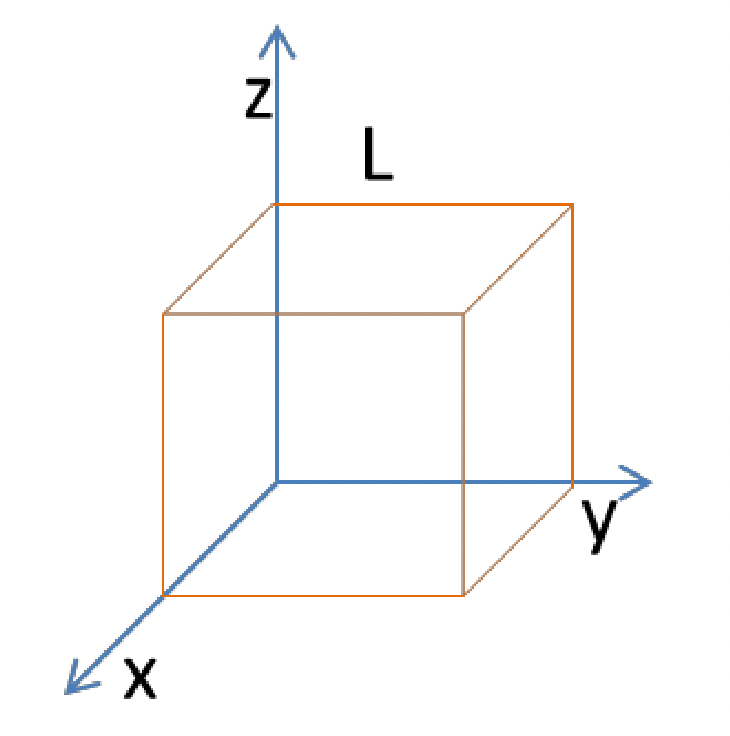
\includegraphics{figs/cube-fermion-gas1}
%	\caption{Fermi surface.}
%	\label{fig:goccia1}
\end{marginfigure}
Gli esponenziali complessi non possono annullarsi per cui è necessario ipotizzare che la funzione d’onda contenga solo le parti sinusoidali o cosinusoidali di tali esponenziali
\begin{equation}
	\psi(\bm{r},t) = A \sin\left(  \frac{1}{\hslash}p_{x}x \right) \sin\left(  \frac{1}{\hslash}p_{y}y \right) \sin\left(  \frac{1}{\hslash}p_{z}z \right) e^{ - \frac{i}{\hslash}Et }
	\label{eq:wave-function-nucleon-fermion-gas-non-normalized}
\end{equation}
In questa forma è agevole imporre l’annullamento della funzione d’onda sulle pareti della cavità nucleare ovvero sui piani $x=0$, $x=L$;  $y=0$, $y=L$; $z=0$, $z=L$.
Ragionando ad esempio lungo la direzione $x$ abbiamo le condizioni
\[
\frac{1}{\hslash} p_{x}x \big|_{x = 0,L} = 0
\]
sempre soddisfatta in $x=0$ e soddisfatta in $x=L$ solo se
\[
\frac{1}{\hslash}p_{x}L = n_{x} \pi \qquad n_{x} = 1,2, \dots, N
\]
Dato che condizioni analoghe si trovano immediatamente anche nelle direzioni y e z, giungiamo alla conclusione che le componenti cartesiane della \emph{quantità di moto} del nucleone soddisfano le seguenti \emph{condizioni di quantizzazione}
\begin{equation}
	p_{x} = n_{x} \frac{\pi \hslash}{L} \quad
	p_{y} = n_{y} \frac{\pi \hslash}{L} \quad
	p_{z} = n_{z} \frac{\pi \hslash}{L} \qquad
	n_{x},n_{y},n_{z} = 1,2, \dots , n
	\label{eq:quantized-momentum-fermions-gas}
\end{equation}
Come anticipato, ciò comporta che pure \emph{l’energia} del nucleone soddisfi la seguente \emph{condizione di quantizzazione}
\begin{equation}
	E = \frac{p^{2}}{2 M} = \frac{1}{2 M} \left( \frac{\pi \hslash}{L} \right)^{2} (n_{x}^{2} + n_{y}^{2}+n_{z}^{2}) \qquad
	n_{x},n_{y},n_{z} = 1,2, \dots , n
	\label{eq:energy-nucleon-fermions-gas}
\end{equation}
dove l'energia considerata è la cinetica in quanto nel modello che stiamo costruendo $ V(r) = 0$ per $ r< R$.
Sostituendo le (\ref{eq:quantized-momentum-fermions-gas}) nella (\ref{eq:wave-function-nucleon-fermion-gas-non-normalized})
ed imponendo la condizione di normalizzazione sul volume nucleare
\begin{gather*}
    \iiint_{V} |\psi(\bm{r},t) |^{2} \, dV = 1 \iff
1 = A^{2} \prod_{i = 1}^{3} \int_{0}^{L} \sin ^{2}\left( n_{x_{i}} \frac{\pi x_{i}}{L} \right) \, dx_{i}\\
    1 = A^{2} \left( \frac{L}{2} \right)^{3} \Longrightarrow A = \sqrt{ \frac{8}{L^{3}} }
\end{gather*}
otteniamo la \textbf{funzione d’onda del nucleone nel volume nucleare cubico di lato L}
\begin{equation}
	\psi(\bm{r},t) = \sqrt{ \frac{8}{L^{3}}} \sin\left( n_{x} \frac{\pi x}{L} \right) \sin\left( n_{y} \frac{\pi y}{L} \right)
	\sin\left( n_{z} \frac{\pi z}{L} \right) e^{ -\frac{i}{\hslash}Et }
	\label{eq:wave-function-nucleon-fermion-gas-normalized}
\end{equation}
Si comprende allora che gli stati quantomeccanici del nucleone vanno a costituire una \emph{sequenza discreta e numerabile di stati univocamente identificati da una terna ordinata di numeri naturali (non nulli e positivi)} $n_x, n_y, n_z$  \emph{detti numeri quantici dello stato}.

\subsection{Nucleoni e principio di esclusione} \label{sec:nucleoni-principio-di-esclusione}
%
%Trovata l’espressione degli stati quantomeccanici di un generico nucleone nella cavità nucleare, vogliamo ora calcolare \emph{il numero di stati che possiedono una energia minore o uguale ad un certo prefissato valore}.
%Con tutta evidenza - dato il legame esistente tra energia e quantità di moto – ciò equivale a calcolare il numero di stati che possiedono un modulo della quantità di moto minore od uguale ad un certo prefissato valore.
%
%Premesso che il calcolo si base sulla stessa tecnica applicata a suo tempo al caso della radiazione elettromagnetica di cavità, si comincia \emph{introducendo uno spazio tridimensionale i cui punti rappresentano i vettori della quantità di moto che avranno così proiezioni} $p_x, p_y \ \text{e} \ p_z$.
%
%Tenendo conto delle relazioni di quantizzazione della quantità di moto (\ref{eq:quantized-momentum-fermions-gas}), si comprende immediatamente che – in tale spazio – i valori delle quantità di moto accessibili al nucleone si collocano nel primo ottante sulle intersezioni di un grigliato tridimensionale di passo $\frac{\pi \hslash}{L}$.
%A ciascuna di tali intersezioni corrisponde anche una determinata terna ordinata di numeri quantici $n_{x}, n_{y}$ e $n_{z}$ e, con essa, un determinato stato quantomeccanico.
%
Prima proseguire sono necessarie alcune precisazioni.
A rigore, la funzione d’onda (\ref{eq:wave-function-nucleon-fermion-gas-normalized}) descrive lo stato di uno dei nucleoni del nucleo dato che soddisfa le condizioni imposte dal potenziale nucleare medio. Lo stato del nucleo nel suo complesso é allora descritto dal prodotto tensoriale di ‘A’ funzioni del tipo (\ref{eq:wave-function-nucleon-fermion-gas-normalized}), ciascuna con la propria terna $n_{x}, n_{y}$ e $n_{z}$ di \emph{numeri quantici di stato}. Ciò premesso, si capisce che non fa differenza descrivere lo stato del nucleo nel modo suddetto oppure immaginare di utilizzare una sola funzione d’onda del tipo (\ref{eq:wave-function-nucleon-fermion-gas-normalized}) specificando però per ciascuna terna $n_{x},n_{y},n_{z}$ il numero di nucleoni che vi risiedono. Questo seconda possibilità, basata sui \emph{numeri di occupazione} dello stato, risulta particolarmente utile nel caso dei fermioni dove il principio di esclusione limita i numeri di occupazione ai soli valori ‘0’ ed ‘1’. Nel prosieguo interpreteremo la funzione d’onda in questo modo.

Fatta questa precisazione possiamo proseguire ricordando che, in accordo con i principi generali della meccanica quantistica, la funzione d’onda (\ref{eq:wave-function-nucleon-fermion-gas-normalized}) descrive nel modo più completo possibile lo stato del nucleo per cui è attraverso di essa che si possono calcolare tutte le grandezze fisiche d’interesse. Nel prosieguo deriveremo la \emph{distribuzione energetica cumulativa} dei nucleoni, necessarie per calcolare le \emph{energie medie dei nucleoni} a loro volta necessarie per il calcolo delle \emph{energie di legame}. Vediamo di cosa si tratta.

Per cominciare domandiamoci quale sia \emph{il numero di stati quantomeccanici che possiedono una energia minore o uguale ad un certo prefissato valore}.
\begin{marginfigure}
	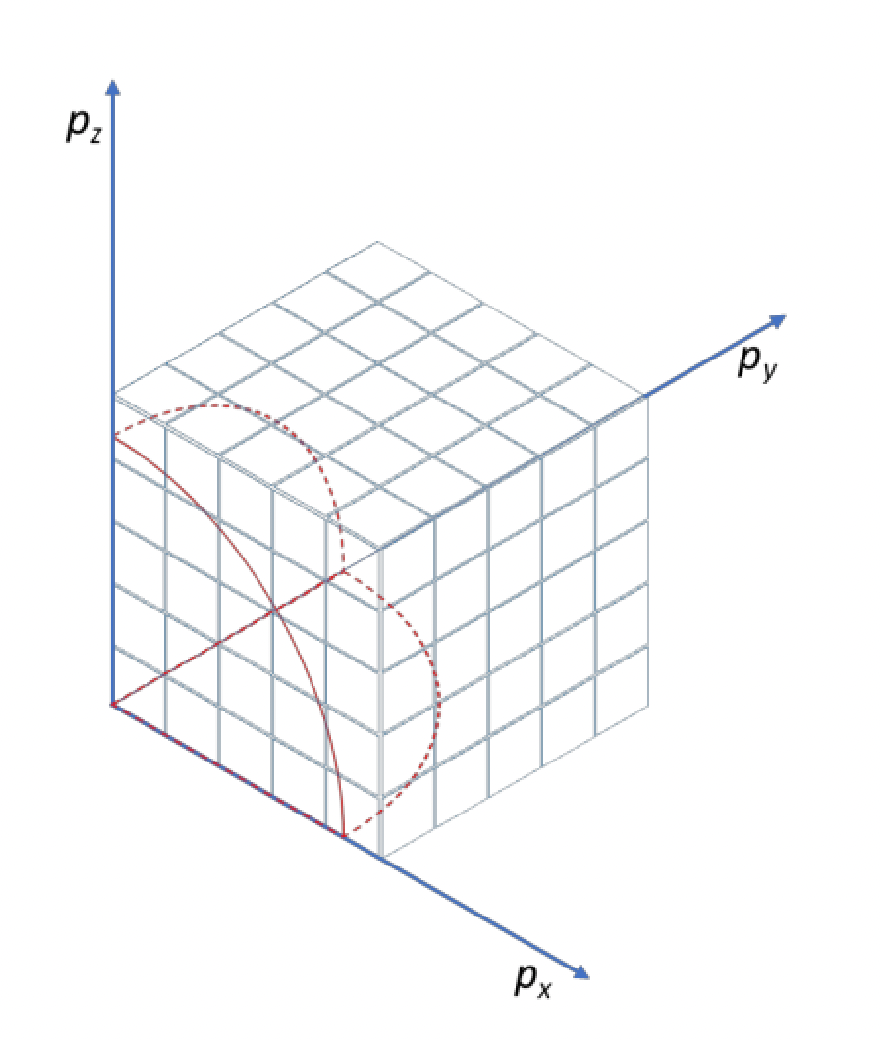
\includegraphics{figs/cube-fermion-gas2}
	%%\caption{Fermi surface.}%%
%  \label{fig:goccia1}
\end{marginfigure}
Dato il legame esistente tra energia e quantità di moto, si deve calcolare il numero di stati aventi modulo della quantità di moto minore od uguale ad un certo prefissato valore.

Utilizzando una tecnica impiegata nel caso della radiazione elettromagnetica di cavità, introduce lo \emph{spazio tridimensionale delle quantità di moto} di assi $p_{x}, p_{y}$ e $p_{z}$. Tenendo conto delle relazioni di quantizzazione (\ref{eq:quantized-momentum-fermions-gas}), si comprende immediatamente che i valori delle quantità di moto accessibili al nucleone si collocano nell’ottante positivo dello spazio (data la positività di $n_{x}, n_{y}$ e $n_{z}$ ), sulle intersezioni di un grigliato tridimensionale di passo $\frac{\pi \hbar}{L}$.
A ciascuna di tali intersezioni corrisponde una determinata terna ordinata di numeri quantici $n_{x}, n_{y}$ e $n_{z}$ e, con essa, un determinato stato quantomeccanico (\ref{eq:wave-function-nucleon-fermion-gas-normalized}).


Ciò premesso, si capisce che \textit{il numero di stati quantomeccanici aventi modulo della quantità di moto uguale o inferiore ad un prefissato valore}
$\tilde{p}$ è approssimativamente uguale al quoziente tra il volume dell’ottante di sfera di raggio $\tilde{p}$ ed il volumetto cubico del grigliato
\[
n_{s} = \frac{1}{8} \frac{ \frac{4}{3} \pi \tilde{p}^{3}}{\left( \frac{\pi \hslash}{L} \right)^{3}} = \frac{L^{3}}{6 \pi^{2}\hslash^{3}}\tilde{p}^{3}
\]
dove abbiamo posto $L^{3} = V$.
Un attimo di attenzione chiarisce che tale formula in realtà sovrastima il numero di stati quantomeccanici.
Infatti, tutti gli statti quantomeccanici interni all’ottante sferico di cui sopra, ma giacenti sui tre piani coordinati $p_x=0, p_y=0$ e $p_z=0$, annullano la funzione d’onda (\ref{eq:wave-function-nucleon-fermion-gas-normalized}) e corrispondono pertanto ad un medesimo stato quantico che deve essere contato una volta sola. E’ facile capire che il numero di tali stati è uguale al quoziente tra le aree dei tre quarti di circonferenza di raggio $\tilde{p}$ dell’ottante sferico e l’areola quadrata associata a ciascuno stato quantomeccanico
\[
n_{0} = \frac{3 \frac{1}{4} \pi \tilde{p}^{2}}{\left( \frac{\pi \hslash}{L} \right)^{2}} = \frac{3}{4} \frac{L^{2}}{\pi \hslash^{2}} \tilde{p}^{2} =
\frac{S}{8\pi \hslash^{2}}\tilde{p}^{2}
\]
dove, nell’ultimo passaggio, abbiamo introdotto la superficie della scatola cubica $S = 6 L^{2}$.
Troviamo allora che \textit{ il numero di stati quantici tali che} $0< | p|<\tilde{p}$  in realtà vale
\[
n_{s} = \frac{V}{6 \pi^{2}\hslash^{3}} \tilde{p}^{3} - \frac{S}{8\pi \hslash^{2}}\tilde{p}^{2}
\]
Dato che, secondo il principio di esclusione di Pauli, ciascuno stato quantistico della funzione d’onda orbitale può alloggiare al massimo due fermioni identici (uno per ciascuno dei due stati di spin del nucleone descritti da uno spinore che abbiamo omesso) concludiamo che \textbf{il numero di neutroni o protoni identici che possono essere contenuti nel volume nucleare V di superficie S con valore massimo dell’impulso} $P_F$ è dato dalla espressione seguente
\begin{marginfigure}
	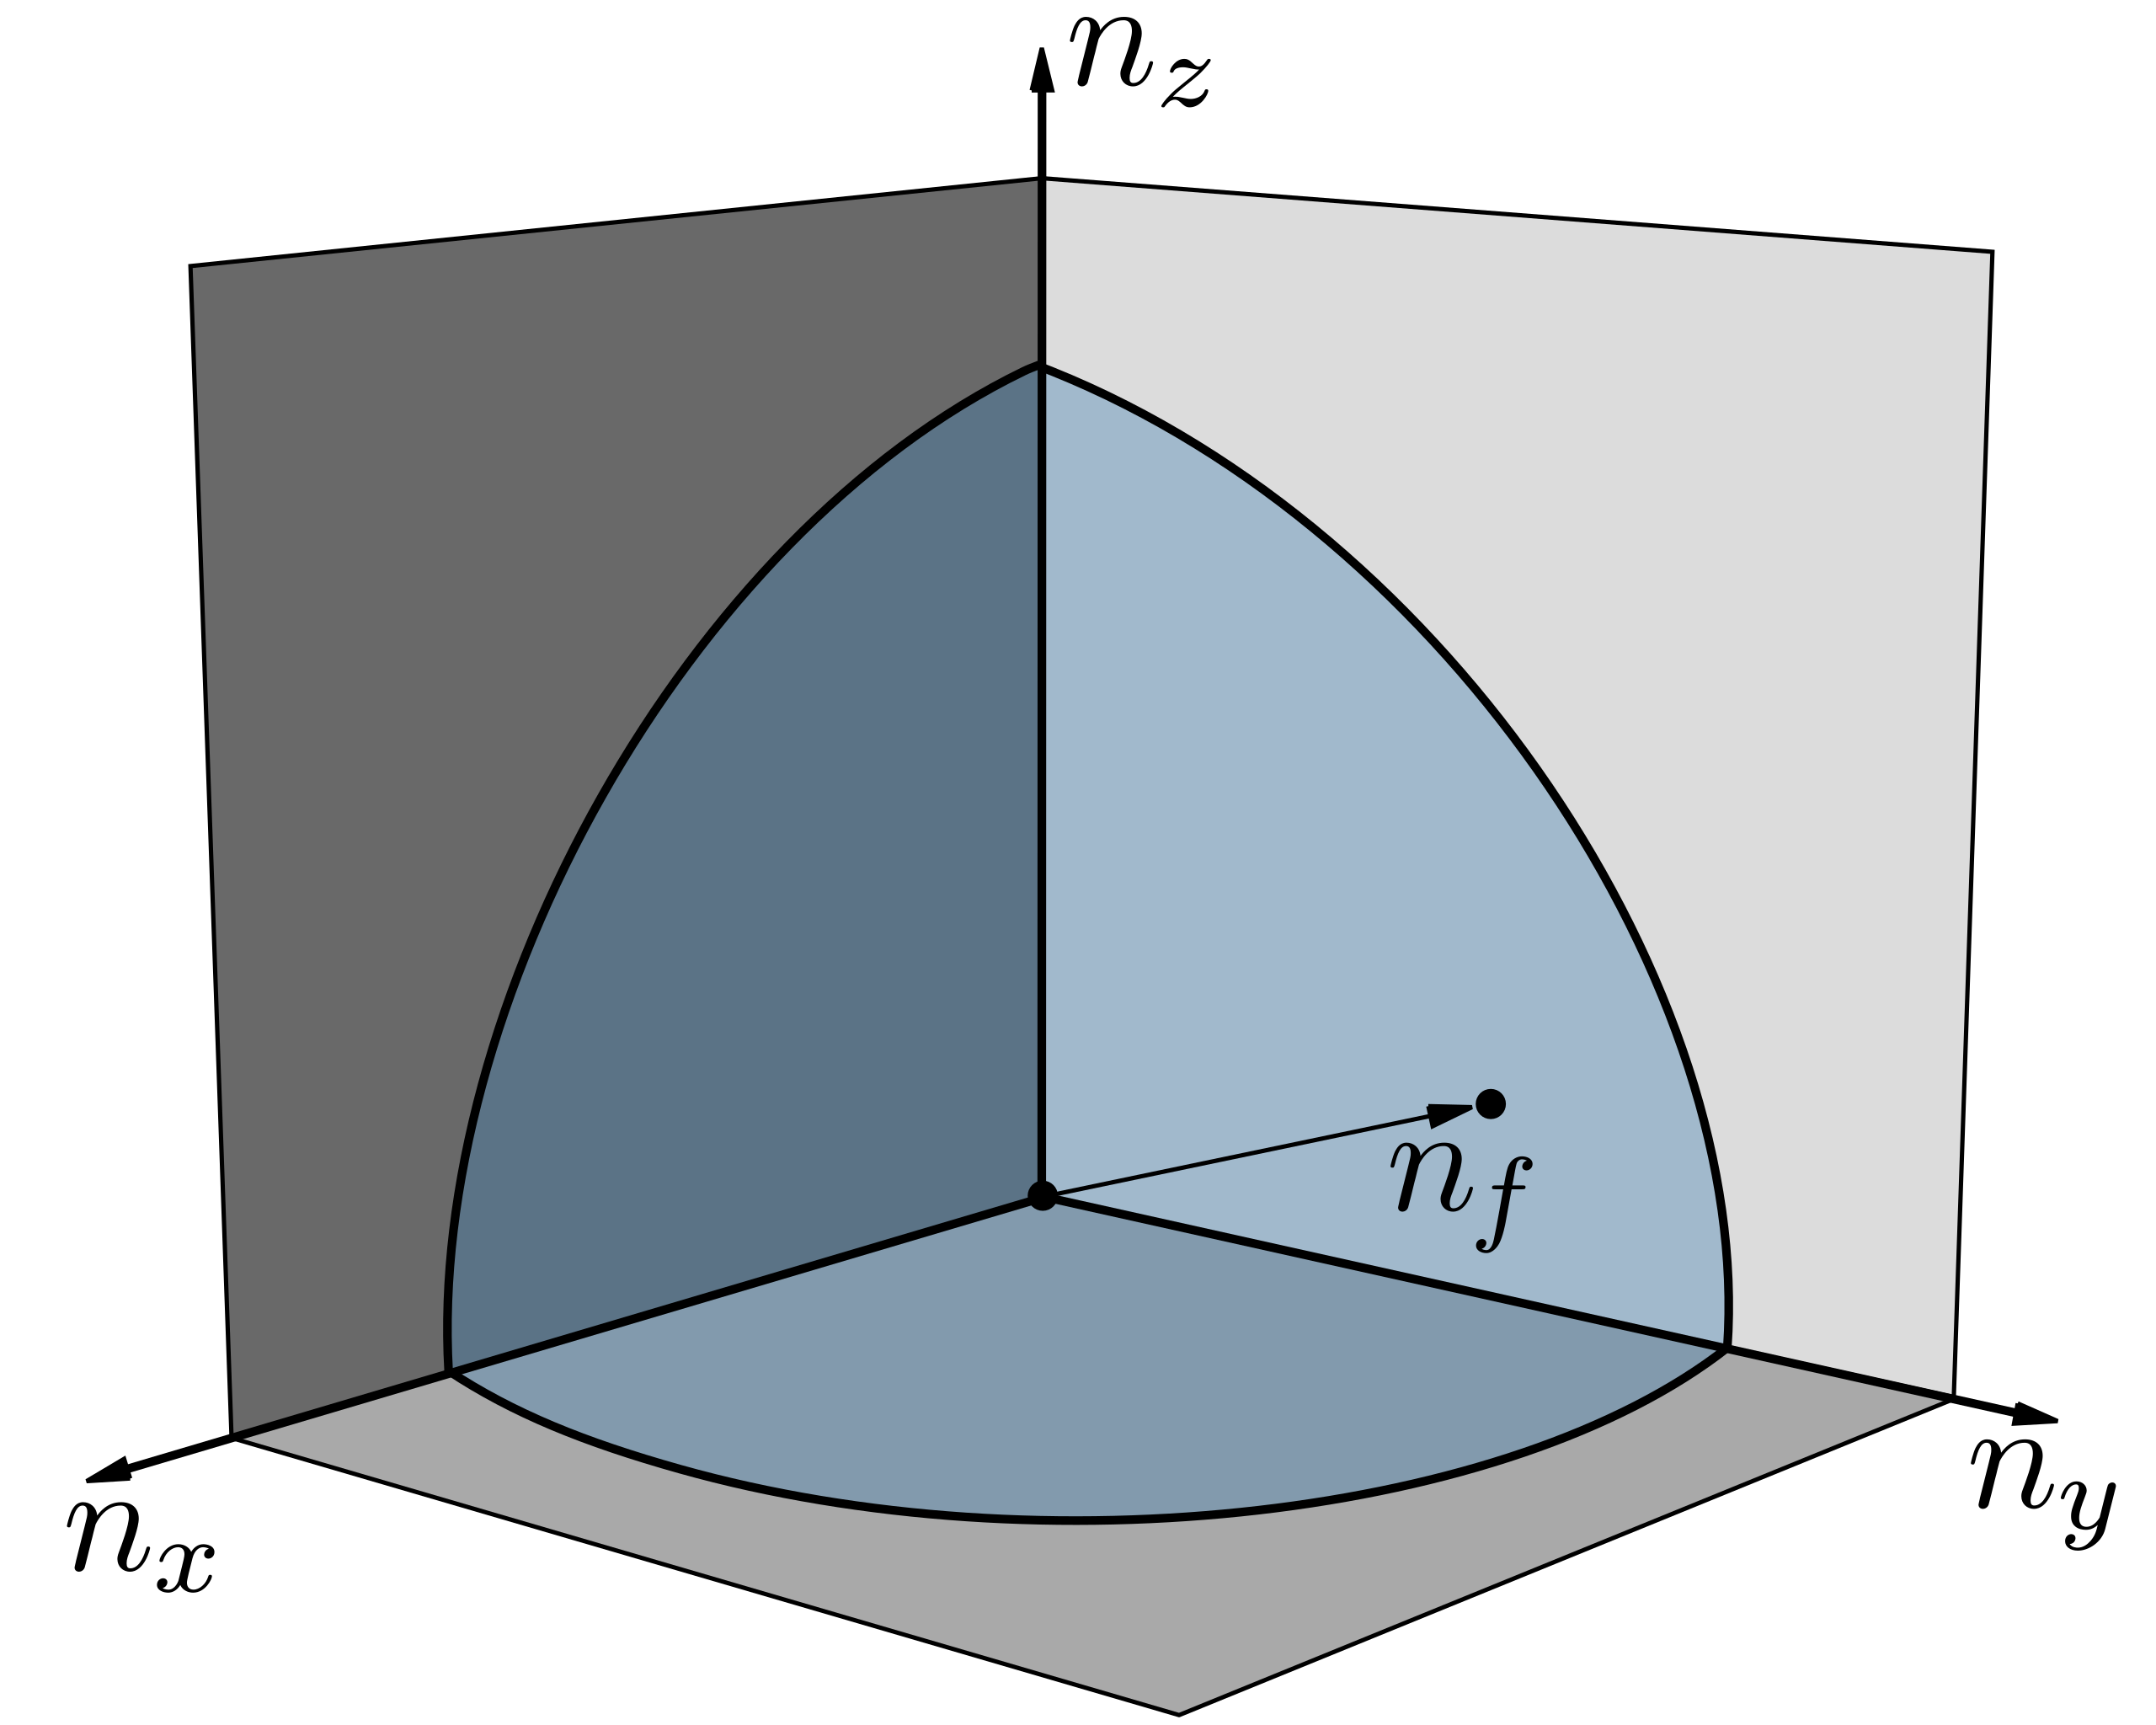
\includegraphics{figs/Fermi-surface}
	\caption{Fermi surface.}
%	\label{fig:goccia1}
\end{marginfigure}
\begin{equation}
	n_{F} = \frac{V P_{F}^{3}}{3 \pi^{2}\hslash^{3}} \left( 1 - \frac{3\pi \hslash}{4} \frac{S}{VP_{F}} \right)
	\label{eq:fermions-number-specified-volume-momentum}
\end{equation}

Essa costituisce la formula fondamentale del modello a gas di fermioni, base di ogni successivo sviluppo del modello stesso.
La (\ref{eq:fermions-number-specified-volume-momentum}) permette di stimare immediatamente alcune grandezze fisiche fondamentali del modello. Trascurando il termine di superficie che si può mostrare essere assi più piccolo di quello di volume, ricaviamo l’espressione \emph{dell’impulso di fermi in funzione del numero di fermioni nucleari}( tenendo conto del fatto che $\frac{\hslash S}{V} \ll 1$)
\begin{equation}
	P_{F} \simeq \hslash \left(\frac{3\pi^{2}n_{F}}{V} \right)^{1/3}
	\label{eq:fermi-momentum-estimate}
\end{equation}
Le ipotesi di \emph{stabilità} del nuclide e dell'occupazione dello \emph{stato di minima energia} si traducono in
\[
	V \simeq \frac{4}{3}\pi r_{0}^{3}A \quad e \quad n_{p}\simeq n_{s} \simeq \frac{A}{2}
\]
per cui usando la (\ref{eq:fermi-momentum-estimate}) possiamo ottenere una stima del valore \textbf{dell’impulso di Fermi} dei protoni e neutroni nucleari
\[
P_{F} = \left( \frac{9\pi}{8} \right)^{1/3} \frac{\hslash}{r_{0}} \simeq 1.52 \frac{\hslash}{1.2 \times \frac{1}{200}\frac{\hslash c}{MeV}} \simeq 254 \frac{MeV}{c}
\]
Dunque, \emph{nel nucleo prossimo allo stato fondamentale, esiste una frazione di nucleoni con un impulso piuttosto rilevante}. Inoltre, \emph{l’impulso di Fermi dei protoni e neutroni risulta essere indipendentemente dal tipo e dimensioni del nucleo}, un fatto che non ci sorprende solo a posteriori.
\bigskip

E’ immediato allora stimare la \textbf{energia cinetica di Fermi} dei protoni e neutroni nucleari
\begin{equation}
	E_{F} = \frac{P_{F}^{2}}{2M_{n,p}} \simeq 34 \, MeV
	\label{eq:fermi-kinetic-energy-estimate}
\end{equation}
%Nel caso del nuclepiù semplice ($H$) si avrà che
%%%TODO 20/12/22 niccolozanotti: farsi spiegare da marco cosa scrivere qui
ed anche la \textbf{profondità della buca di potenziale nucleare} che sarà approssimativamente uguale alla somma della energia di Fermi con la energia media di separazione dei nucleoni che vale circa $8 \, MeV$
(vedi Fig.~\ref{fig:en-legame-graph})
\begin{equation}
	V_{0} \simeq E_{F} + \frac{B}{A} \simeq (34 + 8)\, MeV \simeq 42 \, MeV
   \label{eq:}
\end{equation}
entrambi indipendenti da A \emph{e dunque approssimativamente valide per tutti i nuclei}.

\subsection{L'espressione dell'energia di legame}\label{subsec:energia-di-legame-fermions-gas}

Si noti che l’energia cinetica dei nucleoni non è molto inferiore alla profondità della buca (è inferiore di 8 MeV appunto) per cui \emph{il nucleo è un insieme di nucleoni debolmente legati}.

Nel caso dei nuclei stabili pesanti dobbiamo tenere conto che il numero di neutroni eccede quello dei protoni per cui dalla (\ref4.30) e (\ref4.31) otteniamo \emph{che l’impulso e la energia di Fermi dei neutroni supera quello dei protoni}
\[
P_{F}^n > P_{F}^p \qquad E_{F}^n > E_{F}^p
\]
e così pure per la (\ref4.32) \emph{la profondità della buca di potenziale dei neutroni supera quella dei protoni}
\[
V_{0}^n > V_{0}^p
\]
Se ora teniamo conto che i protoni - a causa della carica elettrica che possiedono - sono soggetti ad un potenziale repulsivo coulombiano sostanzialmente apprezzabile solo
quando quello nucleare si azzera, abbiamo che i potenziali complessivi di
neutroni e protoni devono avere l’andamento approssimato mostrato in Figura~\ref{fig:fermi-gas-model-potential-scheme}.

\begin{figure}
	\centering
	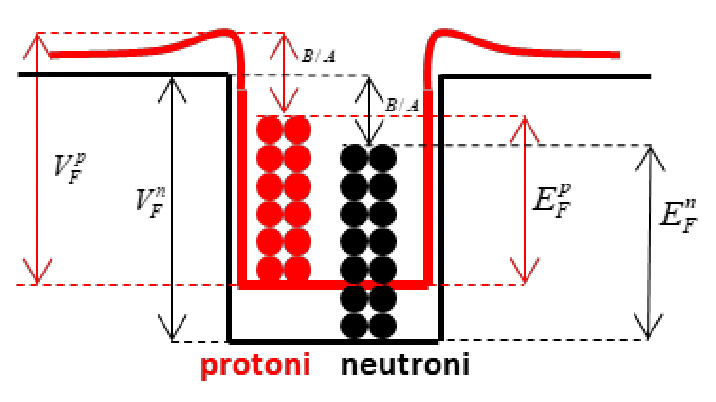
\includegraphics{../figs/fermi-gas-model-potential-scheme}
	\caption{Scheme of Fermi gas model potential.}
	\label{fig:fermi-gas-model-potential-scheme}
\end{figure}

Queste considerazioni chiariscono le linee di ragionamento che possono condurre alla costruzione della \emph{formula della energia di legame basata sul modello a gas di fermioni}.

Un \textbf{neutrone porta un contributo medio alla energia di legame nucleare} pari alla differenza tra la profondità della buca di potenziale e la sua energia cinetica media
\[
b_{n} = V_{0} - \langle T_{n} \rangle
\]
Per un protone si deve ragionare allo stesso modo aggiungendovi però la repulsione coulombiana che rende la buca del potenziale totale meno profonda.
La repulsione coulombiana media per protone ha la seguente espressione (8-1 Feynman\cite{FeynLect2})
\[
	\langle V_{coul} \rangle = \frac{1}{Z} \mathlarger{\sum}_{\substack{j,k=1 \\ j \neq k, \,j > k  }}^{Z} \frac{e^{2}}{4 \pi \epsilon_{0}r_{jk}}\]
e dipende dalla disposizione spaziale dei protoni.
Ipotizzando una distribuzione spazialmente uniforme (problema della sfera uniformemente carica) otteniamo
\[
U_{coul}^{tot} = \frac{3}{5} \frac{e^{2}}{4 \pi \epsilon_{0}} \frac{Z^{2}}{R} = \frac{3}{5} \frac{e^{2}}{4 \pi \epsilon_{0} \hslash c} \hslash c \frac{Z^{2}}{R} = \frac{3}{5} \alpha \hslash c \frac{Z^{2}}{R}
\]
dove $\alpha \simeq \frac{1}{137}$ è la \emph{costante adimensionale di struttura fina} e $R$ è il raggio della distribuzione sferica di carica ovvero il raggio nucleare.
Invocando un ragionamento già fatto per il modello a goccia quando si è parlato del termine coulombiano (si veda (\ref{eq:work-to-seperate-uniformly-distributed-protons})) nel nostro modello la precedente si riscrive come
\[
U_{coul}^{tot} = \frac{3}{5} \alpha \hslash c \frac{Z (Z-1)}{R} \ \cdot
\]
Possiamo ora scrivere il \emph{contributo medio del protone alla energia di legame nucleare} $b_{p}$\sidenote
{
Osserviamo che $ b_n$ e $ b_p$ sono stati stimati teoricamente a partire dal modello a gas di Fermi e non tramite
considerazioni sul difetto di massa come in precedenza. Di fatto si vuole migliorare il precedente modello fenomenologico
(a goccia) cercando di ricavare la dipendenza di $ B$ da $ A$ e $ Z$.
}
\begin{gather*}
    \langle U^{tot}_{coul} \rangle = \frac{U^{tot}_{coul}}{Z}\\
    b_{p} = V_{0} - \langle T_{p} \rangle  - \frac{1}{Z}
\end{gather*}
Tenendo ora conto espressione e dell’analoga per i neutroni possiamo comporre la seguente \textbf{espressione della energia di legame nucleare}
\begin{equation}
	B = N b_{n} + Z b_{p} = A V_{0} - N \langle T_{n} \rangle - Z \langle T_{p} \rangle - \frac{3}{5} \alpha \hslash c \frac{Z(Z-1)}{R}
	\label{eq:binding-energy-fermi-gas-model}
\end{equation}


\subsection{Il calcolo dell'energia di legame}\label{sec:calcolo-energia-legame-fermions-gas}

Per sviluppare l'enegia di legame è ora necessario calcolare le energie cinetiche medie dei neutroni e protoni nucleari.
Si ha
\[
\langle T \rangle = \frac{\sum_{i}T_{i}n_{i}'}{\sum_{i}n_{i}'} \quad , \quad n_{i}' \circeq \Delta_{i}n = n_{i+1}- n_{i} \quad
i = 0, \dots, \bar{n}
\]
dove $\bar{n}$ è il numero di protoni/neutroni propri del livello di Fermi.
Ora, immaginando un addensamento di strati energetici tra $0$ ed il livello di fermi $E_{F}$, possiamo effettuare il passaggio al continuo
\begin{equation}
	\langle T \rangle = \fraclarg{\int_{0}^{P_{F}} \frac{p^{2}}{2m} \, dn}{\int_{0}^{P_{F}}  \, dn }
	\label{eq:average-kinetic-energy-nucleons}
\end{equation}
dove $dn$ indica il numero di neutroni/protoni con impulso compreso tra $p$ e $p+dp$.

Il differenziale della (\ref{eq:fermions-number-specified-volume-momentum}) fornisce tale numero di neutroni/protoni
\[
dn = \frac{V}{\pi^{2}\hbar^{3}} p^{2}dp - \frac{S}{2 \pi \hbar^{2}} pdp
\]
che può essere sostituito nella (\ref{eq:average-kinetic-energy-nucleons}) ottenendo
\begin{align*}
    \langle T \rangle &= \fraclarg{\int_{0}^{P_{F}} \frac{p^{2}}{ 2m}\left(\frac{V}{\pi^{2}\hbar^{3}} p^{2}dp - \frac{S}{2 \pi \hbar^{2}} pdp \right)  }{\frac{V}{3\pi^{2}\hbar^{3}} P_{F}^{3} - \frac{S}{4 \pi \hbar^{2}} P_{F}^{2} }
    = \fraclarg{\frac{VP_{F}^{5}}{10m\pi^{2}\hbar^{3}} - \frac{SP_{F}^{4}}{16m\pi \hbar^{2}}}{\frac{V}{3\pi^{2}\hbar^{3}} P_{F}^{3} - \frac{S}{4 \pi \hbar^{2}} P_{F}^{2}}\\
    &= \fraclarg{\frac{VP_{F}^{5}}{10m \pi^{2}\hbar^{3}}\left( 1 - \frac{10m\pi^{2}\hbar^{3}}{VP_{F}^{5}} \frac{SP_F^{4}}{16 m \pi \hbar^{2}} \right)}{\frac{VP_{F}^{3}}{3\pi^{2}\hbar^{3}}\left( 1 - \frac{3\pi^{2}\hbar^{3}}{VP_{F}^{3}} \frac{S}{4 \pi \hbar^{2}}P_{F}^{2} \right)}
	= \frac{3}{10 \,m}P_{F}^{2} \fraclarg{1 - \frac{5\pi \hbar}{8} \frac{S}{VP_{F}}}{1 - \frac{3\pi \hbar}{4} \frac{S}{VP_{F}}}
\end{align*}
Tramite un'espansione in serie di Taylor al primo ordine
\begin{gather*}
    a = \frac{5\pi \hbar}{8 P_{F}} \quad b = \frac{3\pi \hbar}{4 P_{F}} \quad x = \frac{S}{V}\\
    \frac{1-ax}{1-bx} = 1 + (b-a)x + O(x^{2})
\end{gather*}
otteniamo
\begin{align}
    \langle T \rangle &\simeq  \frac{3P_{F}^{2}}{10 \, m} \left( 1 - \frac{\frac{5\pi \hbar}{8}S}{VP_{F}}+ \frac{3\pi \hbar}{4} \frac{S}{V P_{F}} \right) \nonumber\\
     &= \frac{3}{10 \, m}P_{F}^{2} \left( 1 + \frac{\pi\hbar S}{8 V P_{F}} \right)
	\label{eq:approximated-kinetic-energy-nucleons}
\end{align}
Tenendo conto solo del termine dominante, possiamo migliorare la stima (\ref{eq:fermi-kinetic-energy-estimate}) del \emph{valore della energia cinetica media dei neutroni e protoni nucleari}
\[
\langle T \rangle \simeq \frac{3}{10 \, m} P_{F}^{2} \simeq \frac{3}{5}E_{F} \simeq \frac{3 \times 34}{5} \simeq 21 \, MeV
\]
Ritornando alla (\ref{eq:approximated-kinetic-energy-nucleons}) è chiaro che si vuole disporre di una espressione della energia cinetica media dove compaiano i parametri nucleari $(N, Z, V, S)$ e non il valore dell’impulso di Fermi.
Ciò significa che conviene eliminare la variabile $P_{F}$ nella (\ref{eq:approximated-kinetic-energy-nucleons}) utilizzando la (\ref{eq:fermions-number-specified-volume-momentum}), che nel contesto delle approssimazioni utilizzate\sidenote{
Per arrivare a (\ref{eq:approximated-kinetic-energy-nucleons}) si è sviluppato in serie di Taylor. Tale serie risulta convergente nel caso in cui $| b| < \frac{1}{| x|}$, cioè se
	\[
		\frac{3\pi \hbar}{4} \frac{S}{V P_{F}} \ll 1
	\]
	condizione che permette di compiere l'approssimazione svolta.
} si approssima a
\[
n_{F} =  \frac{VP_{F}^{3}}{3 \pi^{2}\hbar^{3}} \left( 1 -  \frac{3\pi \hbar}{4} \frac{S}{V P_{F}} \right) \simeq \frac{VP_{F}^{3}}{3 \pi^{2} \hbar^{3}}
\]
da cui
\begin{equation}
	P_{F} = \left( \frac{3\pi^{2}\hbar^{3}n_{F}}{V} \right)^{1/3}
	\label{eq:fermi-momentum-in-terms-of-fermi-number}
\end{equation}
Sostituendo (\ref{eq:fermi-momentum-in-terms-of-fermi-number}) in (\ref{eq:approximated-kinetic-energy-nucleons})
\[
\langle T \rangle \simeq \frac{3}{10 \, m}     P_{F} = \left( \frac{3\pi^{2}\hbar^{3}n_{F}}{V} \right)^{2/3} + \frac{3}{80 \, m} \frac{\pi \hbar S}{V}\left( \frac{3\pi^{2}\hbar^{3}n_{F}}{V} \right)^{1/3}
\]
da cui, infine, \emph{l’espressione cercata della energia cinetica media dei fermioni in funzione dei parametri nucleari}
\[
\langle T \rangle \simeq \frac{9\hbar^{2}}{10 \, m} \left( \frac{\pi^{4}n_{F}^{2}}{3 V^{2}}\right)^{1/3}  + \frac{9\hbar^{2}}{80 \, m}\left( \frac{\pi^{5}n_{F}}{9V^{4}} \right)^{1/3}S
\]
Sostituendo questa espressione nella (\ref{eq:binding-energy-fermi-gas-model}) ci avviamo verso l’espressione finale della energia di legame
\begin{align*}
	B \simeq A V_{0} &- N \left[ \frac{9\hbar^{2}}{10\, m} \left( \frac{\pi^{4}N^{2}}{3 V^{2}} \right)^{1/3} + \left( \frac{9\hbar^{2}}{80 \, m} \frac{\pi^{5}N}{9V^{4}} \right)^{1/3}S \right] \\
	& -Z \left[ \frac{9\hbar^{2}}{10\, m} \left( \frac{\pi^{4}Z^{2}}{3 V^{2}} \right)^{1/3} + \left( \frac{9\hbar^{2}}{80 \, m} \frac{\pi^{5}Z}{9V^{4}} \right)^{1/3}S \right] \\
	& - \frac{3}{5} \alpha \hbar c \frac{Z(Z-1)}{R} \\
	= AV_{0} & - \frac{9\hbar^{2}}{80 \, m}\left( \frac{\pi^{5}}{9} \right)^{1/3} \frac{S(N^{4/3}+Z^{4/3})}{V^{4/3}} \\
	&- \frac{9\hbar^{2}}{10 \, m} \left( \frac{\pi^{4}}{3} \right)^{1/3} \frac{N^{5/3}+Z^{5/3}}{V^{2/3}} - \frac{3}{5} \alpha \hbar c \frac{Z(Z-1)}{R}
\end{align*}
dove abbiamo introdotto una unica massa per protone e neutrone.
Ora dobbiamo ricordare che nel nucleo $V, R, N$ e $Z$ sono variabili correlate
\[
V = \frac{4}{3} \pi r_{0}^{3} \qquad S = 4\pi r_{0}^{2}A^{2/3} \qquad R = r_{0}A^{1/3}
\]
per cui sostituendo nella precedente
\begin{align*}
	AV_{0} &- \frac{9 \hbar^{2}}{80 \, m} \left( \frac{\pi^{5}}{9} \right)^{1/3} \frac{4 \pi r_{0}^{2}A^{2/3}(N^{4/3}+Z^{4/3})}{\left( \frac{4}{3} \pi r_{0}^{3} A\right)^{4/3}} \\
	&- \frac{9 \hbar^{2}}{10 \, m} \left( \frac{\pi^{4}}{3} \right)^{1/3} \frac{N^{5/3}+Z^{5/3}}{\left( \frac{4}{3} \pi r_{0}^{3} A\right)^{2/3}} - \frac{3}{5} \alpha \hbar c \frac{Z(Z-1)}{r_{0}A^{1/3}} \\
	AV_{0} &- \frac{9 \hbar^{2}}{80 \, m} \left( \frac{\pi^{5}}{9} \right)^{1/3} \frac{3^{4/3}}{ 4^{1/3}\pi^{1/3}r_{0}^{2}} \frac{N^{4/3}+Z^{4/3}}{A^{2/3}} \\
	&- \frac{9 \hbar^{2}}{10 \, m} \left( \frac{\pi^{4}}{3} \right)^{1/3} \frac{3^{2/3}}{ 4^{2/3}\pi^{2/3}r_{0}^{2}}\frac{N^{5/3}+Z^{5/3}}{ A^{2/3}} - \frac{3}{5} \alpha \hbar c \frac{Z(Z-1)}{r_{0}A^{1/3}} \\
	= AV_{0} &- \frac{9 \hbar^{2}}{80 \, m} \left( \frac{9\pi^{4}}{4} \right)^{1/3} \frac{3^{4/3}}{ 4^{1/3}\pi^{1/3}r_{0}^{2}} \frac{N^{4/3}+Z^{4/3}}{A^{2/3}} \\
	&- \frac{9 \hbar^{2}}{10 \, mr_{0}^{2}} \left( \frac{3\pi^{2}}{16} \right)^{1/3} \frac{N^{5/3}+Z^{5/3}}{ A^{2/3}} - \frac{3}{5} \alpha \hbar c \frac{Z(Z-1)}{r_{0}A^{1/3}} \\
\end{align*}
da cui infine
\begin{align}
	B = A V_{0} &- \frac{9\hbar^{2}}{80 mr_{0}^{2}} \left( \frac{3\pi^{2}}{2} \right)^{2/3}\frac{N^{4/3}+Z^{4/3}}{A^{2/3}} \nonumber\\
	&- \frac{3\hbar^{2}}{10 mr_{0^{2}}}\left( \frac{9\pi}{4} \right)^{2/3} \frac{N^{5/3}+Z^{5/3}}{A^{2/3}} - \frac{3}{5} \alpha \hbar c \frac{Z(Z-1)}{r_{0}A^{1/3}}
	\label{eq:intermediate-calc-binding-energy-fermi-gas}
\end{align}
Per avere questa espressione in una forma confrontabile con l’espressione empirica della energia di legame nucleare conviene passare alle variabili
\[
A=(N+Z) \quad\delta = (N-Z) \qquad N = \frac{A+\delta}{2} \quad Z = \frac{A- \delta}{2}
\]
tenendo anche presente che la variabile $\delta$, nel caso dei nuclei stabili, tende ad essere piccola.

Possiamo allora approssimare con il seguente sviluppo in serie, trattenendo anche i termini del secondo ordine
\[
(1 + x)^{\alpha} \simeq 1 + \alpha x + \frac{1}{2} \alpha (\alpha - 1)x^{2}
\]
I termini in N, Z e A della (\ref{eq:intermediate-calc-binding-energy-fermi-gas}) prendono allora le seguenti forme
\begin{align*}
	\frac{N^{5/3}+Z^{5/3}}{ A^{2/3}} & = \frac{(A+\delta)^{5/3} + (A-\delta)^{5/3}}{2^{5/3} A^{2/3}} = \frac{A}{2^{5/3}} \left[ \left( 1+\frac{\delta}{A} \right)^{5/3} +\left( 1 - \frac{\delta}{A} \right)^{5/3} \right] \\
	& \simeq \frac{A}{2^{5/3}} \left[ 1 + \frac{5}{3}\left( \frac{\delta}{A} \right) + \frac{5}{9} \left( \frac{\delta}{A} \right)^{2} + 1 - \frac{5}{3} \left( \frac{\delta}{A} \right) + \frac{5}{9} \left( \frac{\delta}{A} \right)^{2} \right] \\
	& = \frac{A}{2^{2/3}}  \left[ 1+\frac{5}{9} \left( \frac{\delta}{A} \right)^{2} \right]
	\simeq \frac{A}{2^{2/3}} \left[ 1 + \frac{5}{9} \left( \frac{N-Z}{A} \right)^{2} \right]
\end{align*}
\begin{align*}
	\frac{N^{4/3}+Z^{4/3}}{ A^{2/3}} & = \frac{(A+\delta)^{4/3} + (A-\delta)^{4/3}}{2^{4/3} A^{2/3}} = \frac{A}{2^{4/3}} \left[ \left( 1+\frac{\delta}{A} \right)^{4/3} +\left( 1 - \frac{\delta}{A} \right)^{4/3} \right] \\
	& \simeq \frac{A}{2^{4/3}} \left[ 1 + \frac{4}{3}\left( \frac{\delta}{A} \right) + \frac{2}{9} \left( \frac{\delta}{A} \right)^{2} + 1 - \frac{4}{3} \left( \frac{\delta}{A} \right) + \frac{2}{9} \left( \frac{\delta}{A} \right)^{2} \right] \\
	& = \frac{A}{2^{1/3}}  1+\frac{5}{9} \left( \frac{\delta}{A} \right)^{2}
	\simeq \frac{A}{2^{2/3}} \left[ 1 + \frac{2}{9} \left( \frac{N-Z}{A} \right)^{2} \right]
\end{align*}
Sostituendo $N=A-Z$ otteniamo infine le seguenti espressioni
\begin{align*}
	\frac{N^{5/3}+Z^{5/3}}{ A^{2/3}} &\simeq \frac{A}{2^{2/3}} \left[ 1 + \frac{5}{9} \left( \frac{A-2Z}{A} \right)^{2} \right]\\
	\frac{N^{4/3}+Z^{4/3}}{ A^{2/3}} &\simeq \frac{A}{2^{2/3}} \left[ 1 + \frac{2}{9} \left( \frac{A-2Z}{A} \right)^{2} \right]
\end{align*}
che sostituite nella (\ref{eq:intermediate-calc-binding-energy-fermi-gas}) permettono di sviluppare ulteriormente
l’espressione della energia di legame
\begin{align*}
	B \simeq A V_{0} &- \frac{9\hbar^{2}}{80 mr_{0}^{2}}\left( \frac{3\pi^{2}}{2} \right)^{2/3} \frac{A^{2/3}}{2^{1/3}}  \left[ 1+ \frac{2}{9} \left( \frac{A-2Z}{A} \right)^{2} \right] \\
	&- 3 \frac{\hbar^{2}}{10 m r_{0}^{2}} \left( \frac{9\pi}{4} \right)^{2/3} \frac{A}{2^{2/3}}  \left[ 1 + \frac{5}{9} \left( \frac{A-2Z}{A} \right)^{2} \right] - \frac{3 \alpha \hbar c}{5 r_{0}} \frac{Z(Z-1)}{A^{1/3}} \\
	AV_{0} &- \frac{9\hbar^{2}}{80mr_{0}^{2}} \left( \frac{3\pi^{2}}{2\sqrt{ 2 }} \right)^{2/3} A^{2/3} - \frac{\hbar^{2}}{\textcolor{cyan}{40} m r_{0}^{2}} \left( \frac{3\pi^{2}}{2\sqrt{ 2 }} \right)^{2/3} \frac{(A-2Z)^{2}}{A^{4/3}} \\
	&- \frac{3\hbar^{2}}{10mr_{0}^{2}} \left( \frac{9\pi}{8} \right)^{2/3}A - \frac{\hbar^{2}}{6mr_{0}^{2}} \left( \frac{9\pi}{8} \right)^{2/3} \frac{(A-2Z)^{2}}{A} - \frac{3 \alpha \hbar c}{5 r_{0}} \frac{Z(Z-1)}{A^{1/3}}
\end{align*}
che ora riscriviamo nella sua forma finale
\begin{align}
		B &\simeq \left[ V_{0} - \frac{3\hbar^{2}}{10mr_{0}^{2}} \left( \frac{9\pi}{8} \right)^{2/3} \right] A - \left[ \frac{9\hbar^{2}}{80mr_{0}^{2}} \left( \frac{3\pi^{2}}{2\sqrt{ 2 }} \right)^{2/3} \right]A^{2/3}
	- \frac{3 \alpha \hbar c}{5 r_{0}} \frac{Z(Z-1)}{A^{1/3}} \nonumber \\
	&- \left[ \frac{\hbar^{2}}{6mr_{0}^{2}} \left( \frac{9\pi}{8} \right)^{2/3}  \right]\frac{(A-2Z)^{2}}{A}
	- \left[ \frac{\hbar^{2}}{\textcolor{cyan}{40} m r_{0}^{2}} \left( \frac{3\pi^{2}}{2\sqrt{ 2 }} \right)^{2/3} \right] \frac{(A-2Z)^{2}}{A^{4/3}}
	\label{eq:binding-energy-expression-fermi-gas-model}
\end{align}


Abbiamo così ottenuto l’espressione della \textbf{energia di legame nucleare nell’ambito del modello a gas di fermioni}.

Si noti che i coefficienti dei termini in $A$ e $Z $dipendono - oltre che da costanti fisiche ben note - da due soli parametri nucleari:
la profondità della buca di potenziale $V_{0}$ ed il raggio del nucleone $r_{0}$ confermando la notevole capacità preditiva del modello. 
Fatto ancor più rilevante, vengono correttamente previsti i termini di volume, superficie, coulombiano e asimmetria della 
espressione del modello a goccia (\ref{eq:weizsacker-formula}):
\begin{align*}
	a_{v} &= V_{0} - 3 \frac{\hbar^{2}}{10 m r_{0}^{2}} \left( \frac{9\pi}{8} \right)^{2/3} \\
	a_{s} &= \frac{9\hbar^{2}}{80 m r_{0}^{2}} \left(  \frac{3\pi^{2}}{2\sqrt{ 2 }} \right)^{2/3} \\
	a_{c} &= \frac{3 \alpha \hbar c}{5 r_{0}} \\
	a_{a} &= \frac{\hbar^{2}}{6 m r_{0}^{2}} \left(\frac{9\pi}{8} \right)^{2/3}
\end{align*}
Tali termini vengono così ricondotti ai principi generali della meccanica quantistica e possono ora fondarsi su di un meccanismo fisico di validità generale.

Ad esempio, tenendo presente il procedimento seguito, possiamo verificare che i termini di volume e superficie sono essenzialmente dovuti alla quantizzazione degli stati dei nucleoni a seguito del loro confinamento all’interno del volume nucleare.

Il termine coulombiano è trattato allo stesso modo del modello a goccia.

Il termine di asimmetria, invece, è ricondotto al principio di esclusione di Pauli e dunque ad uno dei fatti più profondi della meccanica quantistica: nello stato nucleare di minima energia risulta energeticamente conveniente
legare tra loro numeri confrontabili di protoni e neutroni piuttosto che soli neutroni, spiegando così una delle proprietà più controintuitive dei nuclei.
Se si tiene poi conto della mutua repulsione dei protoni si capisce anche la tendenza a legare numeri di neutroni eccedenti rispetto ai protoni.

Meno fortuna ha il termine di accoppiamento.
D’altra parte gli ingredienti immessi nel modello non potevano in nessun modo condurre al risultato di una maggiore stabilità dei nuclei pari-pari, un fatto che richiede evidentemente un potenziale più appropriato che tenga conto anche dello spin dei nucleoni.

In generale, il successo del modello a gas di fermioni dimostra che
\emph{la maggior parte delle proprietà dei nuclei in prossimità dello stato fondamentale sono legate alle proprietà
collettive dei nucleoni in condizioni di forte degenerazione piuttosto che alle specifiche proprietà della forza nucleare}
la quale viene riassunta in una semplice forza di contenimento dei nucleoni.

Si può mettere alla prova in modo ancora più severo il modello calcolando esplicitamente i valori dei diversi termini e confrontandoli con quelli empirici.
Sostituendo i valori numerici otteniamo ( i valori sono in $MeV$)
\[
	a_v \simeq 22 \quad
	a_s \simeq 14.6 \quad
	a_c \simeq 0.070 \quad
	a_a \simeq 10.5
\]
Ad esclusione del termine di accoppiamento di cui abbiamo detto, l’accordo è relativamente soddisfacente
(vedi set di valori (\ref{eq:typical-values-drop-model})) ed è assai degno di nota il fatto che tale accordo sia
ottenuto introducendo due soli parametri liberi (la profondità della buca di potenziale nucleare $V_0$
ed il raggio del nucleone $r_0$).
%%%%%%%%%%%%%%%%%%%%%%%%%%%%%%%%%%%%%%%%%%%%%%%%%%%%%%%%%%%%%%%
\section{Il modello a Shell}\label{sec:il-modello-a-shell}

Dobbiamo ora domandarci quale possa essere il motivo del successo solo parziale del modello a gas di Fermi nella descrizione della energia di legame dei nuclei stabili.

Il suo successo è certamente dovuto al fatto che riconosce il \textbf{ruolo determinante giocato dalla meccanica quantistica} che si manifesta
\begin{itemize}
	\item nella discretizzazione degli stati quantomeccanici e delle loro energie;
	\item nella possibilità di collocare in ciascuno stato quantomeccanico un solo nucleone (principio di esclusione di Pauli).
\end{itemize}

Il suo insuccesso, invece, è probabilmente dovuto alla eccessiva \textbf{semplificazione delle forze nucleari} in gioco poiché si ipotizza che le complesse interazioni che ogni nucleone ha con i suoi vicini possano riassumersi in una \textbf{interazione efficace} \emph{dipendente dalla posizione, nulla all’interno del volume nucleare e di modulo assai elevato e centripeta sulla sua superficie} (buca sferica di potenziale). Tali assunzioni devono essere riviste criticamente.

\subsection{Il potenziale nucleare medio}\label{sec:potenziale-nucleare-medio}

Come già osservato quando costruimmo il modello nucleare a gas di fermioni, la risultante delle forze percepita dal singolo nucleone si dovrebbe riassumere in una forza mediamente nulla all’interno del volume nucleare e mediamente non nulla e centripeta in prossimità della superficie nucleare.
Dunque, un potenziale medio a forma di scatola – se assumiamo la descrizione più drastica – o di forma fisicamente più plausibile con variazioni di potenziale meglio raccordate.

Rimandando per ora il problema della forma concreta del potenziale, sappiamo che - sulla base della meccanica quantistica – gli stati quantomeccanici e le energie dei nucleoni soggetti ad un tale potenziale risulteranno discretizzati.
D’altra parte, il principio di Pauli permette di occupare ciascun stato quantomeccanico con un solo nucleone (qualora si tenga conto anche dello spin) per cui su ogni livello energetico potranno risiedere solo un ben definito numero di neutroni e protoni.
Dato che un nucleo nello stato fondamentale possiede la minima energia, deduciamo che i neutroni ed i protoni andranno a riempire dal basso i diversi livelli energetici nucleari fino a raggiungere due livelli massimi detti \emph{livelli di Fermi} in completa analogia con un gas di fermioni degenere alle bassissime temperature.

Ora, immaginiamo che un neutrone (protone) del nucleo collida con un secondo neutrone (protone).
A seguito della collisione il neutrone (protone) dovrebbe variare la propria energia ma, essendo gli stati quantomeccanici dei livelli energetici completamente occupati, tale variazione avverrà solo nel caso in cui l’energia scambiata sia sufficiente a farlo saltare oltre il livello di Fermi (fenomeno chiamato ‘Pauli blocking’).
Dato che nella maggioranza dei casi ciò non avviene, \emph{il moto del neutrone (protone) risulterà essenzialmente imperturbato} come se gli altri neutroni (protoni) non esistessero affatto e si svilupperà seguendo ‘traiettorie’ regolari ben diverse dalle traiettorie degli atomi/molecole di un gas classico continuamente spezzate dalle reciproche collisioni.

A causa del `Pauli blocking’(vedi sidenote pag~\pageref{siden:pauli-blocking}) dunque, \textbf{l’interazione efficace che governa il moto dei nucleoni nel nucleo non è di tipo stocastico ma piuttosto assimilabile ad una forza posizionale descrivibile quindi da un potenziale}.
\bigskip

Verificata la esistenza di un potenziale nucleare si apre il problema della sua forma che non è detto possa ridursi alla buca sferica di potenziale assunta dal modello a gas di fermioni.
Benchè capace di riprodurre alcune importanti proprietà del nucleo, questa ipotesi deve essere sottoposta a verifica sperimentale. \emph{In che modo, allora, si può determinare la forma del potenziale nucleare}?

La forma del potenziale determina il numero di stati quantomeccanici di ogni possibile livello energetico (ovvero il grado di degenerazione) ed anche la loro spaziatura.
D’altra parte il principio di esclusione lascia risiedere un solo nucleone in ogni stato quantomeccanico e dunque un numero di nucleoni pari al grado di degenerazione in ogni livello energetico.
Ciò significa che contando i nucleoni sui diversi livelli energetici possiamo ottenere informazioni stringenti sulla forma del potenziale nucleare. \emph{In che modo allora si possono contare i protoni ed i neutroni alloggiati nei livelli energetici nucleari}?
\begin{marginfigure}
	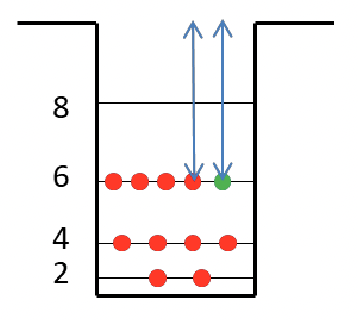
\includegraphics{figs/energy-level-shell1}
	    \caption{Energetic scheme of a nucleon in the mimimum energy state. The highest-energy state is Fermi level.}
	\label{fig:energy-level-shell1}
\end{marginfigure}
Sappiamo che in un nucleo nello stato fondamentale i neutroni ed i protoni vanno ad occupare tutti gli stati quantomeccanici dei diversi livelli energetici fino a raggiungere i rispettivi livelli di Fermi.
\begin{marginfigure}
	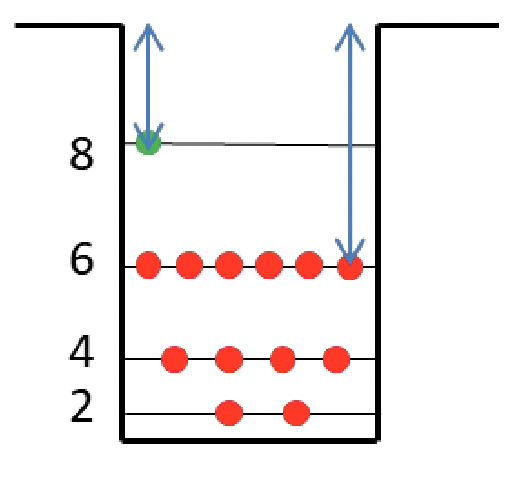
\includegraphics{figs/energy-level-shell2}
	\caption{Energetic scheme of a nucleon in the mimimum energy state. The highest-energy state is Fermi level.}
	\label{fig:energy-level-shell2}
\end{marginfigure}
Dato un nucleo di $N$ neutroni e $Z$ protoni, l’energia che dobbiamo fornire ai neutroni per estrarne uno eguaglia la differenza tra la profondità energetica della buca di potenziale e l’energia del livello di Fermi dei neutroni, ovvero $V_{0}-E_{l}$ (vedi Figura \ref{fig:energy-level-shell1}). Consideriamo allora l’isotopo con N+1 neutroni e Z protoni e domandiamoci ancora una volta quanta energia si debba fornire ai neutroni per estrarne uno dal nucleo. Ci sono due possibili risposte:
\begin{itemize}
	\item se il livello di Fermi dei neutroni del nucleo ($N, Z$) era incompleto, il neutrone in più andrà a collocarsi sullo stesso livello energetico (figura \ref{fig:energy-level-shell1}) e l’energia necessaria sarà ancora $V_{0}-E_{l}$;
    \item se il livello di Fermi dei neutroni del nucleo ($N, Z$) era completo il neutrone in più andrà a collocarsi sul livello energetico successivo e l’energia necessaria avrà un valore inferiore ovvero $V_0 - E_{l+1}$ (vedi Figura \ref{fig:energy-level-shell2}).
\end{itemize}

Giungiamo allora alla conclusione che \emph{le energie di separazione del neutrone in una serie isotopica e del protone in una serie isotonica devono subire bruschi salti in basso in corrispondenza del completamento dei rispettivi livelli energetici nucleari}.
\bigskip

I dati sperimentali delle energie di separazione dei neutroni e protoni nucleari confermano l’andamento previsto.
Nei grafici in Figura~\ref{fig:neutron-separation-energy8-20-82} a lato è infatti possibile osservare diversi salti verso il basso della energia di
separazione del neutrone nel caso delle serie isotopiche dell’Ossigeno, del Calcio e del Piombo che permettono di esplorare
rispettivamente numeri bassi, medi ed elevati di neutroni nucleari.
\begin{marginfigure}
	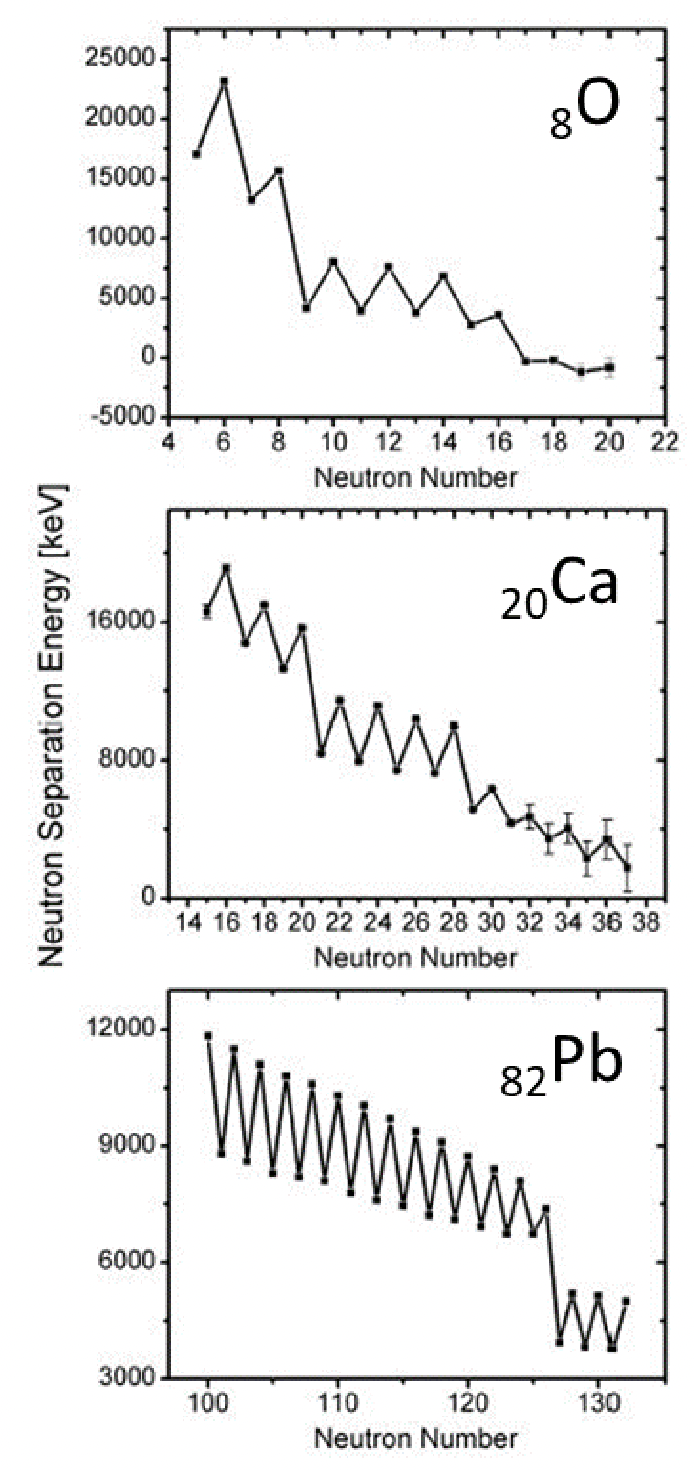
\includegraphics{figs/neutron-separation-energy8-20-82}
	\caption{Energetic scheme of a nucleon in the mimimum energy state. The highest-energy state is Fermi level.}
	\label{fig:neutron-separation-energy8-20-82}
\end{marginfigure}
Si vedono chiaramente i completamenti dei livelli energetici nucleari dei neutroni in corrispondenza dei numeri $8$
(ossigeno), $20, 28$ (calcio) e $126$ (piombo).
Dati analoghi mostrano altri completamenti in corrispondenza dei numeri $50$ e $82$.

La stessa serie di numeri può essere ottenuta anche per i protoni dalla analisi dei dati sperimentali sulle serie isotoniche.

In sintesi possiamo affermare che
\emph{i dati sperimentali sulla energia di separazione dei neutroni e dei protoni indicano che i  livelli energetici nucleari (‘shell’ nucleari)
	si completano in corrispondenza dei numeri 8, 20, 28, 50, 82 e 126 detti numeri magici}.
\bigskip

Si pone ora il problema di stabilire se il potenziale nucleare a forma di \textbf{buca sferica infinita} sia in grado di riprodurre i numeri magici nucleari. Premesso che già sappiamo che questo potenziale non è adeguato poiché prevede una energia di separazione infinita per neutroni e protoni, da un punto di vista generale si tratta di \textbf{risolvere l’equazione di Schroedinger} trovando le \textbf{autofunzioni} e gli \textbf{autovalori} dell’\textbf{operatore hamiltoniano} costruito con il potenziale
\[
V(r) =
\begin{cases}
	0 \qquad \ se \quad r <R \\
	+ \infty \quad se \quad r > R
\end{cases}
\]
Adottato un \emph{sistema di coordinate sferiche} e tenuto conto che l’hamiltoniano non contiene termini dipendenti dal tempo, l’equazione di Schroedinger può essere risolta sostituendo la seguente espressione generale della funzione d’onda separata nelle variabili spaziali e nella variabile temporale
\[
\psi(\mathbf{r},t) = \varphi(r, \theta, \phi) e^{ \frac{i}{\hbar} Et}
\]
Dato che il potenziale non dipende dalle variabili angolari, la parte spaziale della funzione d’onda può essere a sua volta separata nelle variabili angolari stesse e nella variabile radiale
\[
\varphi(r, \theta, \phi) = R(r) \Theta(\theta, \phi)
\]
Svolgendo i calcoli è possibile mostrare che \emph{la parte spaziale della funzione d’onda} deve avere la seguente espressione
\[
\varphi (r, \theta, \phi) = j_{l} (kr) Y_{l,m}(\theta,\phi)
\]
dove le $Y_{l,m}(\theta,\phi)$ sono le già viste \emph{armoniche sferiche}, la famiglia di autofunzioni degli operatori quadrato e terza componente del momento angolare che soddisfano le seguenti \emph{equazioni agli autovalori}
\begin{align*}
	L^{2} Y_{l,m} (\theta, \phi) &= l(l+1) \hbar^{2} Y_{l,m}(\theta,\phi) \qquad l = 0,1,2,\dots \\
	L_{z}Y_{l,m}(\theta, \phi) &= m \hbar Y_{l,m}(\theta,\phi) \qquad
	\qquad \ \ \,
	m = -l,-l+1, \dots, l-1,l
\end{align*}
mentre le $j_{l}(kr)$ sono le altrettanto già viste \emph{funzioni di Bessel} dipendenti in questo caso dal numero quantico del momento angolare $l$.

Ora, affinché \emph{la funzione d’onda possa annullarsi in} $r=R$ (si ricordi che è una delle condizioni al contorno della equazione di Schrödinger per questo problema) si deve avere
\[
j_{l}(kR) = 0
\]
da cui otteniamo la seguente condizione
\[
kR = z_{l,n}
\]
dove, $z_{l,n} \ (n= 1,2,3,\dots)$ \emph{descrive la serie infinita di valori crescenti dell’argomento che annullano la funzione di Bessel} $j_{l}(z)$ di ordine $l$ ed $n$ viene detto \emph{numero quantico principale}. Tale relazione conduce evidentemente alla \emph{quantizzazione del modulo del vettore d’onda} $k$
\[
k = \frac{1}{R} z_{l,n}
\]
Dato che nel problema in esame l’energia possiede solo il termine cinetico (U=0 all’interno del volume sferico), sostituendo la precedente relazione giungiamo alla seguente espressione dei \emph{livelli energetici della buca di potenziale sferica infinita}
\begin{equation}
	E = \frac{\hbar^{2}k^{2}}{2m} = \frac{\hbar^{2}}{2mR^{2}}z_{l,n}^{2}
	\label{eq:energy-levels-infinite-spherical-potential-well}
\end{equation}
dalla quale si evince che
\begin{itemize}
	\item l’energia dipende dal numero quantico del momento angolare $l$ e dal numero quantico principale
	$n$ e per ogni fissato $l$ (ordine della funzione di bessel) aumenta con $n$ (termine ennesimo della serie di zeri);
	\item ad ogni valore della energia, ovvero ad ogni coppia di valori di $l$ ed $n$, corrispondono $(2l+1)$ funzioni d’onda
	diverse nella sola parte angolare: $Y_{l,l} \  Y_{l, -l+1} \dots Y_{l,l-1} \ Y_{l,l}$ , fatto che si riassume dicendo
	che il livello energetico $l, n$ ha una degenerazione di ordine $(2l+1)$.
\end{itemize}

Quasi sempre si utilizza la \textbf{notazione atomica} dove il numero quantico $n$ è indicato esplicitamente al primo posto mentre il numero quantico $l$ è indicato al secondo posto per mezzo della convenzione seguente
\[
l = 0 \to s \quad l = 1 \to p \quad l = 2 \to d \quad l = 3 \to f
\quad l = 4 \to g \quad \dots
\]

\begin{table*}[h]
	\begin{tabular}{|ccccccc|}
		\hline
		\multicolumn{7}{|c|}{3Zeros of Bessel’s Functions of the First Kind} \\ \hline
		\multicolumn{1}{|c|}{Number of Zeros} & \multicolumn{1}{c|}{$J_{0}(x)$} & \multicolumn{1}{c|}{$J_{1}(x)$} & \multicolumn{1}{c|}{$J_{2}(x)$} & \multicolumn{1}{c|}{$J_{3}(x)$} & \multicolumn{1}{c|}{$J_{4}(x)$} & $J_{5}(x)$ \\ \hline
		\multicolumn{1}{|c|}{$1$} & \multicolumn{1}{c|}{$2.40483$} & \multicolumn{1}{c|}{$3.83171$} & \multicolumn{1}{c|}{$5.13562$} & \multicolumn{1}{c|}{$6.38016$} & \multicolumn{1}{c|}{$7.58834$} & $8.77148$ \\ \hline
		\multicolumn{1}{|c|}{$2$} & \multicolumn{1}{c|}{$5.52008$} & \multicolumn{1}{c|}{$7.01559$} & \multicolumn{1}{c|}{$8.41724$} & \multicolumn{1}{c|}{$9.76102$} & \multicolumn{1}{c|}{$11.06471$} & $12.3386$ \\ \hline
		\multicolumn{1}{|c|}{$3$} & \multicolumn{1}{c|}{$8.65373$} & \multicolumn{1}{c|}{$10.17347$} & \multicolumn{1}{c|}{$11.61984$} & \multicolumn{1}{c|}{$13.0152$} & \multicolumn{1}{c|}{$14.37254$} & $15.70017$ \\ \hline
		\multicolumn{1}{|c|}{$4$} & \multicolumn{1}{c|}{$11.79153$} & \multicolumn{1}{c|}{$13.32369$} & \multicolumn{1}{c|}{$14.79595$} & \multicolumn{1}{c|}{$16.22347$} & \multicolumn{1}{c|}{$17.61597$} & $18.98013$ \\ \hline
		\multicolumn{1}{|c|}{$5$} & \multicolumn{1}{c|}{$14.93092$} & \multicolumn{1}{c|}{$16.47063$} & \multicolumn{1}{c|}{$17.95982$} & \multicolumn{1}{c|}{$19.40941$} & \multicolumn{1}{c|}{$20.82693$} & $22.2178$ \\ \hline
	\end{tabular}
\end{table*}
Utilizzando allora la formula (\ref{eq:energy-levels-infinite-spherical-potential-well}) e tenendo conto della tabella
qui riportata degli zeri delle funzioni di Bessel otteniamo i
\emph{livelli energetici della buca di potenziale sferica infinita} indicati in figura~\ref{fig:energetic-levels-infinite-potential-well}.
\begin{marginfigure}
	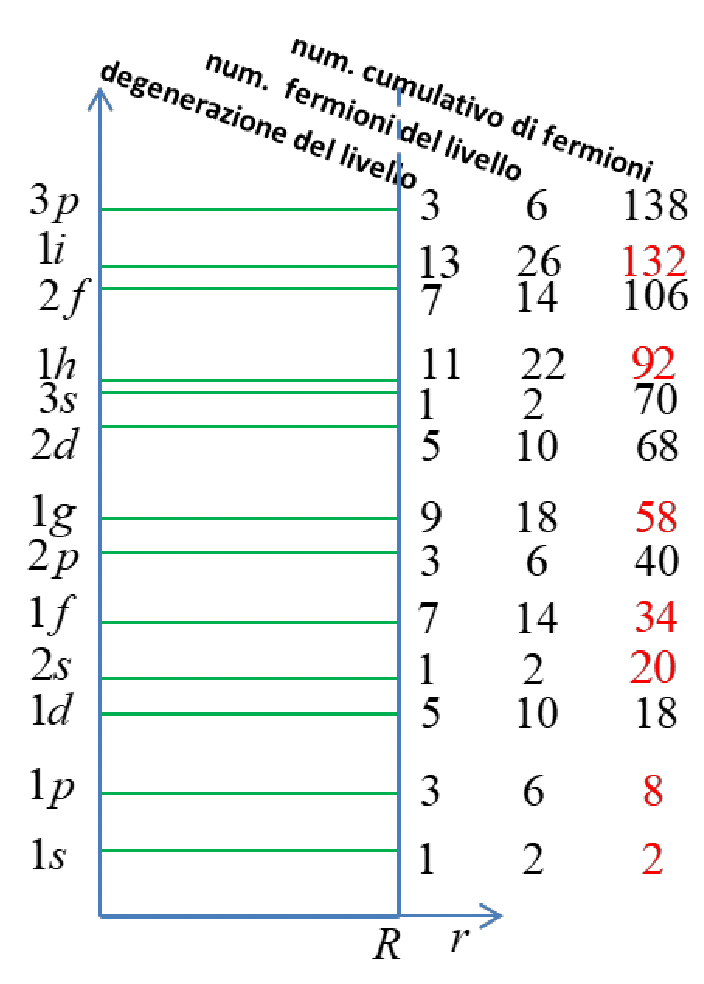
\includegraphics{figs/energetic-levels-infinite-potential-well}
	\caption{Energetic scheme of a nucleon in the mimimum energy state. The highest-energy state is Fermi level.}
	\label{fig:energetic-levels-infinite-potential-well}
\end{marginfigure}
Raggruppando ora i livelli energetici vicini non risolvibili sperimentalmente, possiamo calcolare facilmente i numeri
cumulativi dei diversi gruppi che andranno a costituire i numeri magici della buca di potenziale sferica infinita.

Otteniamo così i numeri marcati in rosso: $2, 8, 20, 34, 58, \dots$.
La serie empirica di numeri magici $8, 20, 28, 50, 82$ e $126$ non è riprodotta in modo soddisfacente per cui dobbiamo concludere che \emph{la forma del potenziale deve essere modificata}.

Una prima ovvia modifica non può essere che quella di richiedere che il potenziale abbia una \emph{profondità finita e non infinita} con una \emph{risalita ripida} ma \emph{non verticale} in $r=R$ così da essere privo di punti assai poco fisici di non derivabilità. Una espressione semplice che soddisfi questi requisiti è data dal \textbf{potenziale di Saxon-Wood}
\[
V_{SW}(r) = -\frac{V_{0}}{1 + \exp{\left( \frac{r-R}{d} \right)}}
\]
dove $V_{0}$ è la profondità della buca di potenziale (dell’ordine di $50 \, MeV$), $R=r_{0}A^{1/3} (r_{0} = 1.24 \, fm)$ è il raggio nucleare e $d = 0.52 \, fm$ lo spessore dell’alone nucleare.
\begin{marginfigure}
	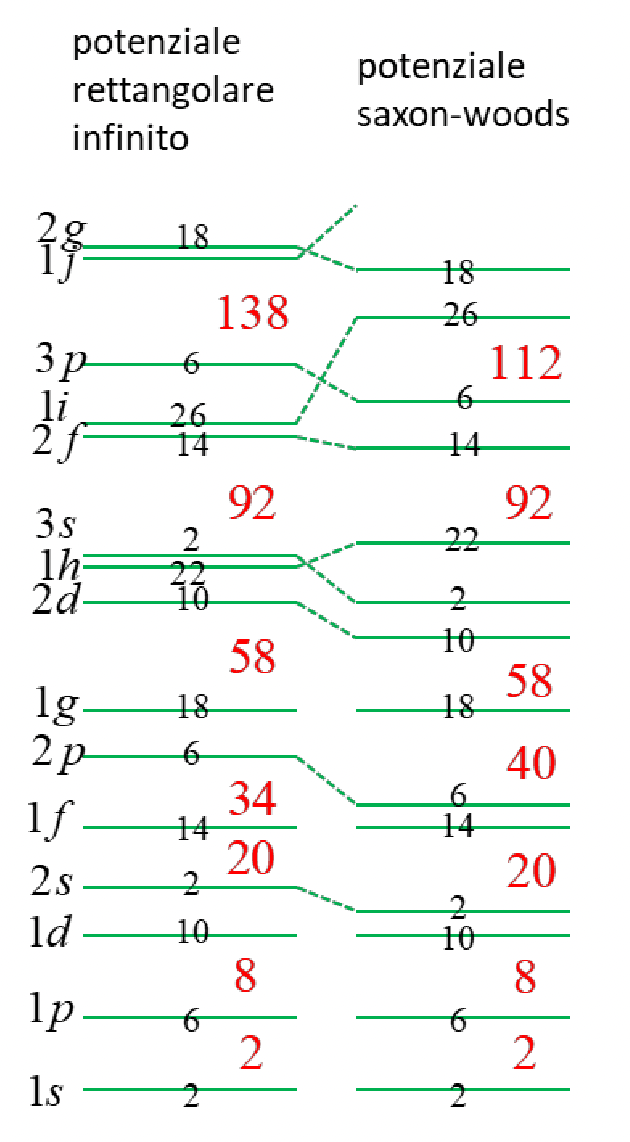
\includegraphics{figs/energetic-levels-sw}
	\caption{Energetic scheme }
	\label{fig:energetic-levels-sw}
\end{marginfigure}
I livelli energetici del potenziale sferico di Saxon-Woods, confrontati con quelli della buca di potenziale sferica infinita, sono mostrati in figura~\ref{fig:energetic-levels-sw}.
Come si vede risultano confermati i numeri magici 2, 8 e 20, quest’ultimo con maggior nettezza del caso precedente, mentre i numeri magici più alti sono errati.
In particolare, il numero magico $28$ sembra davvero problematico poiché nessuno dei livelli successivi al $2s$ porta con sé $8$ nucleoni (il livello $1f$ ne porta ben $14$!).





















































